\section{CuTe in this algebra}\label{sec:cute}\label{sec:idioms}

CuTe lists the modes of a layout with the first varying fastest; we reverse
the list, recursively, and the two then agree as functions on the same
integers. CuTe's $\mathrm{composition}(A,B)$ applies $B$ first and is
$A \circ B$ in our algebra, with $B$ the right operand of
Definition~\ref{def:compose}. We take the four operations in the order of
Section~\ref{sec:intro}, state what each is in our algebra, and name the
documented examples~\cite{cutedocs} on which
the two are checked to agree.

\paragraph{Composition.} In CuTe, $\mathrm{composition}(A,B)$ is the layout
$L$ with $L(c) = A(B(c))$ for every $c \in \mathrm{Coord}(S_B)$. In our
algebra, $A \circ B$ is the map $c \mapsto A(\mathrm{unflatten}_{S_A}(B(c)))$, defined whenever $B$
is a dense bijection onto $[0,\size A)$, and Theorem~\ref{thm:decide} decides
whether it is a layout. For such a $B$, when CuTe's composition exists the
two are the same function, so Theorem~\ref{thm:decide} accepts and returns
the coarsest shape that realizes it. Checked on the three documented examples,
\begin{align*}
\mathrm{composition}\big((6,2){:}(8,2),\,(4,3){:}(3,1)\big)
  &= \big((2,2),3\big){:}\big((24,2),8\big),\\
\mathrm{composition}\big(20{:}2,\,(5,4){:}(4,1)\big) &= (5,4){:}(8,2),\\
\mathrm{composition}\big((10,2){:}(16,4),\,(5,4){:}(1,5)\big)
  &= \big(5,(2,2)\big){:}\big(16,(80,4)\big),
\end{align*}
as functions at every coordinate; in all three $B$ is a dense bijection onto
$[0,\size A)$.

\paragraph{Complement.} In CuTe, $B^{*}_{M}$ is the layout of
Section~\ref{sec:intro}, defined under two divisibility conditions. In our
algebra there is no complement operator. For
$B = (N_0,\dots,N_\alpha){:}(d_0,\dots,d_\alpha)$ the two conditions make
every factor of
$M = d_0 \cdot N_0 \cdot \tfrac{d_1}{N_0 d_0} \cdot N_1 \cdots
\tfrac{M}{N_\alpha d_\alpha}$ an integer. Let $R$ be the shape of these
factors in our order,
$R = \big(\tfrac{M}{N_\alpha d_\alpha},\, N_\alpha,\,
\tfrac{d_\alpha}{N_{\alpha-1}d_{\alpha-1}},\, \dots,\, N_0,\, d_0\big)$,
and let $S$ be $R$ with every entry other than the $N_i$ replaced by $1$.
Then
\[
\divideop\big(\mathrm{canonical}(R),\, S\big) \;=\; \big(B,\ B^{*}_{M}\big)
\]
after dropping entries of size $1$: the tile is $B$ and the rest is its
complement. Whether a given pair $(B, B^{*})$ is a bijection onto $[0,M)$ is
decided by Lemma~\ref{lem:dense}. Checked on the six documented complements:
$\divideop(\mathrm{canonical}(24), (4))$ has tile $4{:}1$ and rest $6{:}4$,
which are $(4{:}1)^{*}_{24}$ and $(6{:}4)^{*}_{24}$;
$\divideop(\mathrm{canonical}((12,2)), (4,1))$ has tile $4{:}2$ and rest
$(3,2){:}(8,1)$, which is $(4{:}2)^{*}_{24} = (2,3){:}(1,8)$; and all six
pairs $(B, B^{*}_{24})$ are bijections onto $[0,24)$.

\paragraph{Division.} In CuTe, $A / B = A \circ (B, B^{*}_{\size A})$. In our
algebra, for a tile given as a shape $S$ with $k_i \mid n_i$, this is $\divideop(A,S)$ of
Section~\ref{sec:ops}, and
\[
\divideop(A, S) \;=\; A \circ \divideop\big(\mathrm{canonical}(S_A),\, S\big),
\]
whose right operand is a regrouping of the identity on $[0,\size A)$ and so a
dense bijection onto it. For a tile given as a layout $B$ it is the composite
$A \circ (B, B^{*}_{\size A})$ itself: $(B, B^{*}_{\size A})$ is a bijection
onto $[0,\size A)$, so Definition~\ref{def:compose} applies with no further
condition. Checked, as functions, on the documented strided tiler,
\[
(4,2,3){:}(2,1,8) \mathbin{/} 4{:}2 =
\big((2,2),(2,3)\big){:}\big((4,1),(2,8)\big).
\]
CuTe's
\texttt{zipped\_divide} groups the result as $((\text{tile}),(\text{rest}))$,
which is the grouping $\divideop$ produces; \texttt{logical\_divide} groups
it per mode, a regrouping of the same layout.

\paragraph{Product.} In CuTe, $A \otimes B = (A, A^{*}_{M} \circ B)$ with
$M = \size A \cdot \cosize B$. In our algebra,
\[
\repeatop(A,B) = (S_B, S_A){:}\big((\cosize A)\,D_B,\ D_A\big).
\]
When $A$ is a dense bijection, $A^{*}_{M} = (\cosize B){:}(\size A)$, so
\[
A \otimes B = \big(A,\ S_B{:}(\size A)\,D_B\big) = \repeatop(A,B).
\]
When $\cosize A > \size A$ the two differ. Take $A = (2,2){:}(4,1)$ and
$B = 6{:}1$. Printed as CuTe prints layouts, one cell per coordinate holding
its address and coloured by the copy it belongs to, $A$ is
\begin{center}
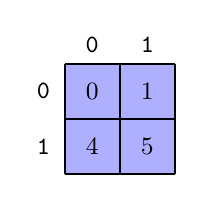
\begin{tikzpicture}[x={(0cm,-0.7cm)},y={(0.7cm,0cm)},every node/.style={minimum size=0.7cm, outer sep=0pt, font=\small}]
\node[fill={rgb,255:red,175;green,175;blue,255}] at (0,0) {0};
\node[fill={rgb,255:red,175;green,175;blue,255}] at (0,1) {1};
\node[fill={rgb,255:red,175;green,175;blue,255}] at (1,0) {4};
\node[fill={rgb,255:red,175;green,175;blue,255}] at (1,1) {5};
\draw[color=black,thick,step=0.7cm,shift={(-0.5,-0.5)}] (0,0) grid (2,2);
\node[anchor=east,minimum size=0pt] at (0,-0.6) {\texttt{0}};
\node[anchor=east,minimum size=0pt] at (1,-0.6) {\texttt{1}};
\node[minimum size=0pt] at (-0.85,0) {\texttt{0}};
\node[minimum size=0pt] at (-0.85,1) {\texttt{1}};
\end{tikzpicture}
\end{center}

and the two products are, with the element $(i,j)$ of $A$ as the row and the
copy $k$ as the column,
\begin{center}
\begin{minipage}[t]{0.48\linewidth}\centering
In CuTe: $A \otimes B$\\[4pt]
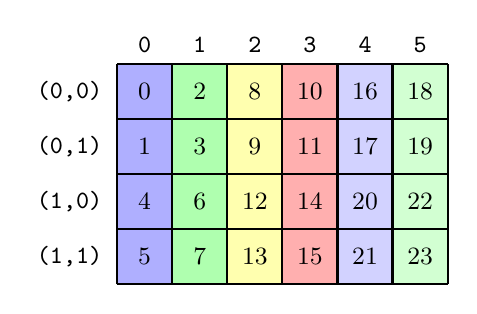
\begin{tikzpicture}[x={(0cm,-0.7cm)},y={(0.7cm,0cm)},every node/.style={minimum size=0.7cm, outer sep=0pt, font=\small}]
\node[fill={rgb,255:red,175;green,175;blue,255}] at (0,0) {0};
\node[fill={rgb,255:red,175;green,255;blue,175}] at (0,1) {2};
\node[fill={rgb,255:red,255;green,255;blue,175}] at (0,2) {8};
\node[fill={rgb,255:red,255;green,175;blue,175}] at (0,3) {10};
\node[fill={rgb,255:red,210;green,210;blue,255}] at (0,4) {16};
\node[fill={rgb,255:red,210;green,255;blue,210}] at (0,5) {18};
\node[fill={rgb,255:red,175;green,175;blue,255}] at (1,0) {1};
\node[fill={rgb,255:red,175;green,255;blue,175}] at (1,1) {3};
\node[fill={rgb,255:red,255;green,255;blue,175}] at (1,2) {9};
\node[fill={rgb,255:red,255;green,175;blue,175}] at (1,3) {11};
\node[fill={rgb,255:red,210;green,210;blue,255}] at (1,4) {17};
\node[fill={rgb,255:red,210;green,255;blue,210}] at (1,5) {19};
\node[fill={rgb,255:red,175;green,175;blue,255}] at (2,0) {4};
\node[fill={rgb,255:red,175;green,255;blue,175}] at (2,1) {6};
\node[fill={rgb,255:red,255;green,255;blue,175}] at (2,2) {12};
\node[fill={rgb,255:red,255;green,175;blue,175}] at (2,3) {14};
\node[fill={rgb,255:red,210;green,210;blue,255}] at (2,4) {20};
\node[fill={rgb,255:red,210;green,255;blue,210}] at (2,5) {22};
\node[fill={rgb,255:red,175;green,175;blue,255}] at (3,0) {5};
\node[fill={rgb,255:red,175;green,255;blue,175}] at (3,1) {7};
\node[fill={rgb,255:red,255;green,255;blue,175}] at (3,2) {13};
\node[fill={rgb,255:red,255;green,175;blue,175}] at (3,3) {15};
\node[fill={rgb,255:red,210;green,210;blue,255}] at (3,4) {21};
\node[fill={rgb,255:red,210;green,255;blue,210}] at (3,5) {23};
\draw[color=black,thick,step=0.7cm,shift={(-0.5,-0.5)}] (0,0) grid (4,6);
\node[anchor=east,minimum size=0pt] at (0,-0.6) {\texttt{(0,0)}};
\node[anchor=east,minimum size=0pt] at (1,-0.6) {\texttt{(0,1)}};
\node[anchor=east,minimum size=0pt] at (2,-0.6) {\texttt{(1,0)}};
\node[anchor=east,minimum size=0pt] at (3,-0.6) {\texttt{(1,1)}};
\node[minimum size=0pt] at (-0.85,0) {\texttt{0}};
\node[minimum size=0pt] at (-0.85,1) {\texttt{1}};
\node[minimum size=0pt] at (-0.85,2) {\texttt{2}};
\node[minimum size=0pt] at (-0.85,3) {\texttt{3}};
\node[minimum size=0pt] at (-0.85,4) {\texttt{4}};
\node[minimum size=0pt] at (-0.85,5) {\texttt{5}};
\end{tikzpicture}
\end{minipage}\hfill
\begin{minipage}[t]{0.48\linewidth}\centering
In our algebra: $\repeatop(A,B)$\\[4pt]
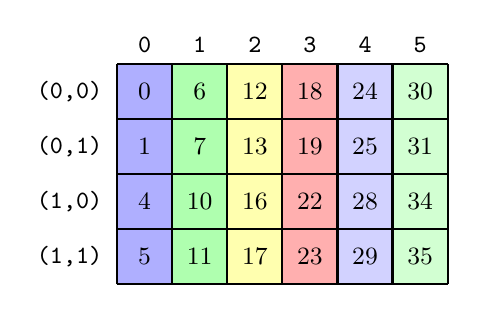
\begin{tikzpicture}[x={(0cm,-0.7cm)},y={(0.7cm,0cm)},every node/.style={minimum size=0.7cm, outer sep=0pt, font=\small}]
\node[fill={rgb,255:red,175;green,175;blue,255}] at (0,0) {0};
\node[fill={rgb,255:red,175;green,255;blue,175}] at (0,1) {6};
\node[fill={rgb,255:red,255;green,255;blue,175}] at (0,2) {12};
\node[fill={rgb,255:red,255;green,175;blue,175}] at (0,3) {18};
\node[fill={rgb,255:red,210;green,210;blue,255}] at (0,4) {24};
\node[fill={rgb,255:red,210;green,255;blue,210}] at (0,5) {30};
\node[fill={rgb,255:red,175;green,175;blue,255}] at (1,0) {1};
\node[fill={rgb,255:red,175;green,255;blue,175}] at (1,1) {7};
\node[fill={rgb,255:red,255;green,255;blue,175}] at (1,2) {13};
\node[fill={rgb,255:red,255;green,175;blue,175}] at (1,3) {19};
\node[fill={rgb,255:red,210;green,210;blue,255}] at (1,4) {25};
\node[fill={rgb,255:red,210;green,255;blue,210}] at (1,5) {31};
\node[fill={rgb,255:red,175;green,175;blue,255}] at (2,0) {4};
\node[fill={rgb,255:red,175;green,255;blue,175}] at (2,1) {10};
\node[fill={rgb,255:red,255;green,255;blue,175}] at (2,2) {16};
\node[fill={rgb,255:red,255;green,175;blue,175}] at (2,3) {22};
\node[fill={rgb,255:red,210;green,210;blue,255}] at (2,4) {28};
\node[fill={rgb,255:red,210;green,255;blue,210}] at (2,5) {34};
\node[fill={rgb,255:red,175;green,175;blue,255}] at (3,0) {5};
\node[fill={rgb,255:red,175;green,255;blue,175}] at (3,1) {11};
\node[fill={rgb,255:red,255;green,255;blue,175}] at (3,2) {17};
\node[fill={rgb,255:red,255;green,175;blue,175}] at (3,3) {23};
\node[fill={rgb,255:red,210;green,210;blue,255}] at (3,4) {29};
\node[fill={rgb,255:red,210;green,255;blue,210}] at (3,5) {35};
\draw[color=black,thick,step=0.7cm,shift={(-0.5,-0.5)}] (0,0) grid (4,6);
\node[anchor=east,minimum size=0pt] at (0,-0.6) {\texttt{(0,0)}};
\node[anchor=east,minimum size=0pt] at (1,-0.6) {\texttt{(0,1)}};
\node[anchor=east,minimum size=0pt] at (2,-0.6) {\texttt{(1,0)}};
\node[anchor=east,minimum size=0pt] at (3,-0.6) {\texttt{(1,1)}};
\node[minimum size=0pt] at (-0.85,0) {\texttt{0}};
\node[minimum size=0pt] at (-0.85,1) {\texttt{1}};
\node[minimum size=0pt] at (-0.85,2) {\texttt{2}};
\node[minimum size=0pt] at (-0.85,3) {\texttt{3}};
\node[minimum size=0pt] at (-0.85,4) {\texttt{4}};
\node[minimum size=0pt] at (-0.85,5) {\texttt{5}};
\end{tikzpicture}
\end{minipage}
\end{center}

In CuTe the copy offsets are $A^{*}_{24} = (2,3){:}(2,8)$, that is
$0, 2, 8, 10, 16, 18$, and
\[
A \otimes B = \big((2,2),(2,3)\big){:}\big((4,1),(2,8)\big)
\]
is a bijection onto $[0,24)$. In our algebra the copy offsets are the multiples of
$\cosize A = 6$, and $\repeatop(A,B) = (6,(2,2)){:}(6,(4,1))$ is injective and
not dense. CuTe's placement is available in our algebra:
$\divideop(\mathrm{canonical}(R), S)$ is the pair $(A, A^{*}_{M})$ of the
complement paragraph, and composing it on the right with
$\repeatop(B, \mathrm{canonical}(S_A))$, which sends $(a,b)$ to $(a, B(b))$,
gives $A \otimes B$ for every dense bijection $B$; for $B = k{:}1$ that
composition is the identity, and for this $A$
\[
A \otimes B = \divideop\big(\mathrm{canonical}((6,4)),\ (2,2)\big).
\]
All of this is checked. With the
operands exchanged and $B$ a dense bijection, $B \otimes A = (B,\
S_A{:}(\size B)\,D_A)$, which is $\interleave(A,B)$ up to the order of the
two coordinate groups. CuTe's \texttt{blocked\_product} and
\texttt{raked\_product} are both $A \otimes B$ with the two coordinate groups
zipped per mode, block index first or copy index first: the same map on
coordinates, regrouped. For $A = 4{:}1$ and $B = 2{:}1$, $A \otimes B =
\repeatop(A,B) = (2,4){:}(4,1)$, \texttt{raked\_product} is $(4,2){:}(1,4)$,
the same map with its two coordinates exchanged, and $B \otimes A =
\interleave(A,B) = (2,4){:}(1,2)$.

\paragraph{Conditions.} CuTe's six conditions exist because its composition
and complement must return a layout, so the operands are checked in advance
for the result to be expressible as one. In our algebra neither operation has
to: a composite is a map, and whether it is a layout is decided afterwards,
for code generation only; and a complement is never formed on its own, it is
the rest of a $\divideop$. So none of the six is checked. What is checked
instead is that the right operand of a composition is a dense bijection onto
the left operand's coordinates, by the stride criterion of
Lemma~\ref{lem:dense}; that a map into logical or thread-value space is a
dense bijection and a map into physical space is alias-free; and the
precondition of each operation, such as $k_i \mid n_i$ for $\divideop$.

\paragraph{Example.} Two hardware instructions and a kernel's use of them.
The thread-value maps are transcribed from the PTX ISA fragment
tables~\cite{ptx}. For
\texttt{mma.m16n8k16}, lane $4g + t_4$ holds four accumulator values
$(v_m, v_n)$, at row $g + 8v_m$ and column $2t_4 + v_n$ of the $16 \times 8$
tile; with the tile row-major,
\[
F_C = \big((8,4),(2,2)\big){:}\big((8,2),(64,1)\big) : \tv \to \logical .
\]
For \texttt{ldmatrix}, lane $4g + q$ holds elements $(g, 2q)$ and $(g, 2q+1)$
of an $8 \times 8$ matrix,
\[
F_{\mathrm{ld}} = \big((8,4),2\big){:}\big((8,2),1\big) : \tv \to \logical .
\]
Printed as CuTe prints thread-value layouts, one cell per element of the tile,
labelled with the lane and value that hold it and coloured by lane:
\begin{center}
\begin{minipage}[t]{0.42\linewidth}\centering
$F_C$: the $16 \times 8$ accumulator\\[4pt]
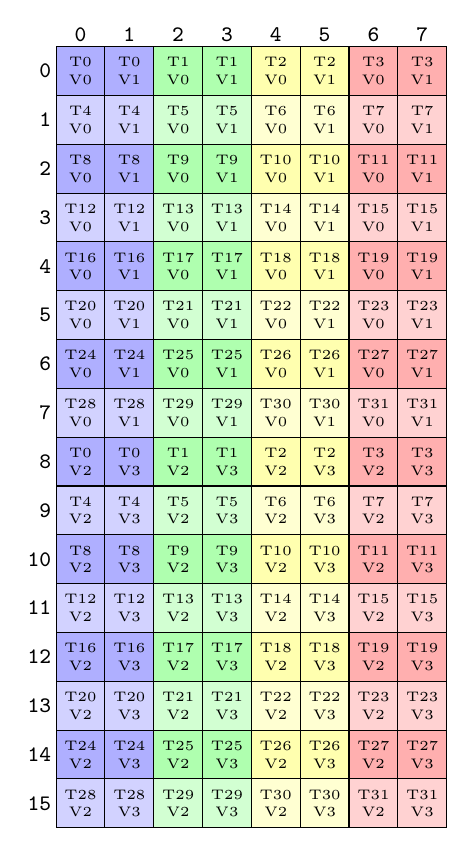
\begin{tikzpicture}[x={(0cm,-0.62cm)},y={(0.62cm,0cm)},every node/.style={minimum size=0.62cm, outer sep=0pt, inner sep=0pt, font=\tiny}]
\node[fill={rgb,255:red,175;green,175;blue,255}] at (0,0) {\shortstack{T0\\V0}};
\node[fill={rgb,255:red,175;green,175;blue,255}] at (0,1) {\shortstack{T0\\V1}};
\node[fill={rgb,255:red,175;green,255;blue,175}] at (0,2) {\shortstack{T1\\V0}};
\node[fill={rgb,255:red,175;green,255;blue,175}] at (0,3) {\shortstack{T1\\V1}};
\node[fill={rgb,255:red,255;green,255;blue,175}] at (0,4) {\shortstack{T2\\V0}};
\node[fill={rgb,255:red,255;green,255;blue,175}] at (0,5) {\shortstack{T2\\V1}};
\node[fill={rgb,255:red,255;green,175;blue,175}] at (0,6) {\shortstack{T3\\V0}};
\node[fill={rgb,255:red,255;green,175;blue,175}] at (0,7) {\shortstack{T3\\V1}};
\node[fill={rgb,255:red,210;green,210;blue,255}] at (1,0) {\shortstack{T4\\V0}};
\node[fill={rgb,255:red,210;green,210;blue,255}] at (1,1) {\shortstack{T4\\V1}};
\node[fill={rgb,255:red,210;green,255;blue,210}] at (1,2) {\shortstack{T5\\V0}};
\node[fill={rgb,255:red,210;green,255;blue,210}] at (1,3) {\shortstack{T5\\V1}};
\node[fill={rgb,255:red,255;green,255;blue,210}] at (1,4) {\shortstack{T6\\V0}};
\node[fill={rgb,255:red,255;green,255;blue,210}] at (1,5) {\shortstack{T6\\V1}};
\node[fill={rgb,255:red,255;green,210;blue,210}] at (1,6) {\shortstack{T7\\V0}};
\node[fill={rgb,255:red,255;green,210;blue,210}] at (1,7) {\shortstack{T7\\V1}};
\node[fill={rgb,255:red,175;green,175;blue,255}] at (2,0) {\shortstack{T8\\V0}};
\node[fill={rgb,255:red,175;green,175;blue,255}] at (2,1) {\shortstack{T8\\V1}};
\node[fill={rgb,255:red,175;green,255;blue,175}] at (2,2) {\shortstack{T9\\V0}};
\node[fill={rgb,255:red,175;green,255;blue,175}] at (2,3) {\shortstack{T9\\V1}};
\node[fill={rgb,255:red,255;green,255;blue,175}] at (2,4) {\shortstack{T10\\V0}};
\node[fill={rgb,255:red,255;green,255;blue,175}] at (2,5) {\shortstack{T10\\V1}};
\node[fill={rgb,255:red,255;green,175;blue,175}] at (2,6) {\shortstack{T11\\V0}};
\node[fill={rgb,255:red,255;green,175;blue,175}] at (2,7) {\shortstack{T11\\V1}};
\node[fill={rgb,255:red,210;green,210;blue,255}] at (3,0) {\shortstack{T12\\V0}};
\node[fill={rgb,255:red,210;green,210;blue,255}] at (3,1) {\shortstack{T12\\V1}};
\node[fill={rgb,255:red,210;green,255;blue,210}] at (3,2) {\shortstack{T13\\V0}};
\node[fill={rgb,255:red,210;green,255;blue,210}] at (3,3) {\shortstack{T13\\V1}};
\node[fill={rgb,255:red,255;green,255;blue,210}] at (3,4) {\shortstack{T14\\V0}};
\node[fill={rgb,255:red,255;green,255;blue,210}] at (3,5) {\shortstack{T14\\V1}};
\node[fill={rgb,255:red,255;green,210;blue,210}] at (3,6) {\shortstack{T15\\V0}};
\node[fill={rgb,255:red,255;green,210;blue,210}] at (3,7) {\shortstack{T15\\V1}};
\node[fill={rgb,255:red,175;green,175;blue,255}] at (4,0) {\shortstack{T16\\V0}};
\node[fill={rgb,255:red,175;green,175;blue,255}] at (4,1) {\shortstack{T16\\V1}};
\node[fill={rgb,255:red,175;green,255;blue,175}] at (4,2) {\shortstack{T17\\V0}};
\node[fill={rgb,255:red,175;green,255;blue,175}] at (4,3) {\shortstack{T17\\V1}};
\node[fill={rgb,255:red,255;green,255;blue,175}] at (4,4) {\shortstack{T18\\V0}};
\node[fill={rgb,255:red,255;green,255;blue,175}] at (4,5) {\shortstack{T18\\V1}};
\node[fill={rgb,255:red,255;green,175;blue,175}] at (4,6) {\shortstack{T19\\V0}};
\node[fill={rgb,255:red,255;green,175;blue,175}] at (4,7) {\shortstack{T19\\V1}};
\node[fill={rgb,255:red,210;green,210;blue,255}] at (5,0) {\shortstack{T20\\V0}};
\node[fill={rgb,255:red,210;green,210;blue,255}] at (5,1) {\shortstack{T20\\V1}};
\node[fill={rgb,255:red,210;green,255;blue,210}] at (5,2) {\shortstack{T21\\V0}};
\node[fill={rgb,255:red,210;green,255;blue,210}] at (5,3) {\shortstack{T21\\V1}};
\node[fill={rgb,255:red,255;green,255;blue,210}] at (5,4) {\shortstack{T22\\V0}};
\node[fill={rgb,255:red,255;green,255;blue,210}] at (5,5) {\shortstack{T22\\V1}};
\node[fill={rgb,255:red,255;green,210;blue,210}] at (5,6) {\shortstack{T23\\V0}};
\node[fill={rgb,255:red,255;green,210;blue,210}] at (5,7) {\shortstack{T23\\V1}};
\node[fill={rgb,255:red,175;green,175;blue,255}] at (6,0) {\shortstack{T24\\V0}};
\node[fill={rgb,255:red,175;green,175;blue,255}] at (6,1) {\shortstack{T24\\V1}};
\node[fill={rgb,255:red,175;green,255;blue,175}] at (6,2) {\shortstack{T25\\V0}};
\node[fill={rgb,255:red,175;green,255;blue,175}] at (6,3) {\shortstack{T25\\V1}};
\node[fill={rgb,255:red,255;green,255;blue,175}] at (6,4) {\shortstack{T26\\V0}};
\node[fill={rgb,255:red,255;green,255;blue,175}] at (6,5) {\shortstack{T26\\V1}};
\node[fill={rgb,255:red,255;green,175;blue,175}] at (6,6) {\shortstack{T27\\V0}};
\node[fill={rgb,255:red,255;green,175;blue,175}] at (6,7) {\shortstack{T27\\V1}};
\node[fill={rgb,255:red,210;green,210;blue,255}] at (7,0) {\shortstack{T28\\V0}};
\node[fill={rgb,255:red,210;green,210;blue,255}] at (7,1) {\shortstack{T28\\V1}};
\node[fill={rgb,255:red,210;green,255;blue,210}] at (7,2) {\shortstack{T29\\V0}};
\node[fill={rgb,255:red,210;green,255;blue,210}] at (7,3) {\shortstack{T29\\V1}};
\node[fill={rgb,255:red,255;green,255;blue,210}] at (7,4) {\shortstack{T30\\V0}};
\node[fill={rgb,255:red,255;green,255;blue,210}] at (7,5) {\shortstack{T30\\V1}};
\node[fill={rgb,255:red,255;green,210;blue,210}] at (7,6) {\shortstack{T31\\V0}};
\node[fill={rgb,255:red,255;green,210;blue,210}] at (7,7) {\shortstack{T31\\V1}};
\node[fill={rgb,255:red,175;green,175;blue,255}] at (8,0) {\shortstack{T0\\V2}};
\node[fill={rgb,255:red,175;green,175;blue,255}] at (8,1) {\shortstack{T0\\V3}};
\node[fill={rgb,255:red,175;green,255;blue,175}] at (8,2) {\shortstack{T1\\V2}};
\node[fill={rgb,255:red,175;green,255;blue,175}] at (8,3) {\shortstack{T1\\V3}};
\node[fill={rgb,255:red,255;green,255;blue,175}] at (8,4) {\shortstack{T2\\V2}};
\node[fill={rgb,255:red,255;green,255;blue,175}] at (8,5) {\shortstack{T2\\V3}};
\node[fill={rgb,255:red,255;green,175;blue,175}] at (8,6) {\shortstack{T3\\V2}};
\node[fill={rgb,255:red,255;green,175;blue,175}] at (8,7) {\shortstack{T3\\V3}};
\node[fill={rgb,255:red,210;green,210;blue,255}] at (9,0) {\shortstack{T4\\V2}};
\node[fill={rgb,255:red,210;green,210;blue,255}] at (9,1) {\shortstack{T4\\V3}};
\node[fill={rgb,255:red,210;green,255;blue,210}] at (9,2) {\shortstack{T5\\V2}};
\node[fill={rgb,255:red,210;green,255;blue,210}] at (9,3) {\shortstack{T5\\V3}};
\node[fill={rgb,255:red,255;green,255;blue,210}] at (9,4) {\shortstack{T6\\V2}};
\node[fill={rgb,255:red,255;green,255;blue,210}] at (9,5) {\shortstack{T6\\V3}};
\node[fill={rgb,255:red,255;green,210;blue,210}] at (9,6) {\shortstack{T7\\V2}};
\node[fill={rgb,255:red,255;green,210;blue,210}] at (9,7) {\shortstack{T7\\V3}};
\node[fill={rgb,255:red,175;green,175;blue,255}] at (10,0) {\shortstack{T8\\V2}};
\node[fill={rgb,255:red,175;green,175;blue,255}] at (10,1) {\shortstack{T8\\V3}};
\node[fill={rgb,255:red,175;green,255;blue,175}] at (10,2) {\shortstack{T9\\V2}};
\node[fill={rgb,255:red,175;green,255;blue,175}] at (10,3) {\shortstack{T9\\V3}};
\node[fill={rgb,255:red,255;green,255;blue,175}] at (10,4) {\shortstack{T10\\V2}};
\node[fill={rgb,255:red,255;green,255;blue,175}] at (10,5) {\shortstack{T10\\V3}};
\node[fill={rgb,255:red,255;green,175;blue,175}] at (10,6) {\shortstack{T11\\V2}};
\node[fill={rgb,255:red,255;green,175;blue,175}] at (10,7) {\shortstack{T11\\V3}};
\node[fill={rgb,255:red,210;green,210;blue,255}] at (11,0) {\shortstack{T12\\V2}};
\node[fill={rgb,255:red,210;green,210;blue,255}] at (11,1) {\shortstack{T12\\V3}};
\node[fill={rgb,255:red,210;green,255;blue,210}] at (11,2) {\shortstack{T13\\V2}};
\node[fill={rgb,255:red,210;green,255;blue,210}] at (11,3) {\shortstack{T13\\V3}};
\node[fill={rgb,255:red,255;green,255;blue,210}] at (11,4) {\shortstack{T14\\V2}};
\node[fill={rgb,255:red,255;green,255;blue,210}] at (11,5) {\shortstack{T14\\V3}};
\node[fill={rgb,255:red,255;green,210;blue,210}] at (11,6) {\shortstack{T15\\V2}};
\node[fill={rgb,255:red,255;green,210;blue,210}] at (11,7) {\shortstack{T15\\V3}};
\node[fill={rgb,255:red,175;green,175;blue,255}] at (12,0) {\shortstack{T16\\V2}};
\node[fill={rgb,255:red,175;green,175;blue,255}] at (12,1) {\shortstack{T16\\V3}};
\node[fill={rgb,255:red,175;green,255;blue,175}] at (12,2) {\shortstack{T17\\V2}};
\node[fill={rgb,255:red,175;green,255;blue,175}] at (12,3) {\shortstack{T17\\V3}};
\node[fill={rgb,255:red,255;green,255;blue,175}] at (12,4) {\shortstack{T18\\V2}};
\node[fill={rgb,255:red,255;green,255;blue,175}] at (12,5) {\shortstack{T18\\V3}};
\node[fill={rgb,255:red,255;green,175;blue,175}] at (12,6) {\shortstack{T19\\V2}};
\node[fill={rgb,255:red,255;green,175;blue,175}] at (12,7) {\shortstack{T19\\V3}};
\node[fill={rgb,255:red,210;green,210;blue,255}] at (13,0) {\shortstack{T20\\V2}};
\node[fill={rgb,255:red,210;green,210;blue,255}] at (13,1) {\shortstack{T20\\V3}};
\node[fill={rgb,255:red,210;green,255;blue,210}] at (13,2) {\shortstack{T21\\V2}};
\node[fill={rgb,255:red,210;green,255;blue,210}] at (13,3) {\shortstack{T21\\V3}};
\node[fill={rgb,255:red,255;green,255;blue,210}] at (13,4) {\shortstack{T22\\V2}};
\node[fill={rgb,255:red,255;green,255;blue,210}] at (13,5) {\shortstack{T22\\V3}};
\node[fill={rgb,255:red,255;green,210;blue,210}] at (13,6) {\shortstack{T23\\V2}};
\node[fill={rgb,255:red,255;green,210;blue,210}] at (13,7) {\shortstack{T23\\V3}};
\node[fill={rgb,255:red,175;green,175;blue,255}] at (14,0) {\shortstack{T24\\V2}};
\node[fill={rgb,255:red,175;green,175;blue,255}] at (14,1) {\shortstack{T24\\V3}};
\node[fill={rgb,255:red,175;green,255;blue,175}] at (14,2) {\shortstack{T25\\V2}};
\node[fill={rgb,255:red,175;green,255;blue,175}] at (14,3) {\shortstack{T25\\V3}};
\node[fill={rgb,255:red,255;green,255;blue,175}] at (14,4) {\shortstack{T26\\V2}};
\node[fill={rgb,255:red,255;green,255;blue,175}] at (14,5) {\shortstack{T26\\V3}};
\node[fill={rgb,255:red,255;green,175;blue,175}] at (14,6) {\shortstack{T27\\V2}};
\node[fill={rgb,255:red,255;green,175;blue,175}] at (14,7) {\shortstack{T27\\V3}};
\node[fill={rgb,255:red,210;green,210;blue,255}] at (15,0) {\shortstack{T28\\V2}};
\node[fill={rgb,255:red,210;green,210;blue,255}] at (15,1) {\shortstack{T28\\V3}};
\node[fill={rgb,255:red,210;green,255;blue,210}] at (15,2) {\shortstack{T29\\V2}};
\node[fill={rgb,255:red,210;green,255;blue,210}] at (15,3) {\shortstack{T29\\V3}};
\node[fill={rgb,255:red,255;green,255;blue,210}] at (15,4) {\shortstack{T30\\V2}};
\node[fill={rgb,255:red,255;green,255;blue,210}] at (15,5) {\shortstack{T30\\V3}};
\node[fill={rgb,255:red,255;green,210;blue,210}] at (15,6) {\shortstack{T31\\V2}};
\node[fill={rgb,255:red,255;green,210;blue,210}] at (15,7) {\shortstack{T31\\V3}};
\draw[color=black,thin,step=0.62cm,shift={(-0.5,-0.5)}] (0,0) grid (16,8);
\node[anchor=east,minimum size=0pt,font=\footnotesize] at (0,-0.6) {\texttt{0}};
\node[anchor=east,minimum size=0pt,font=\footnotesize] at (1,-0.6) {\texttt{1}};
\node[anchor=east,minimum size=0pt,font=\footnotesize] at (2,-0.6) {\texttt{2}};
\node[anchor=east,minimum size=0pt,font=\footnotesize] at (3,-0.6) {\texttt{3}};
\node[anchor=east,minimum size=0pt,font=\footnotesize] at (4,-0.6) {\texttt{4}};
\node[anchor=east,minimum size=0pt,font=\footnotesize] at (5,-0.6) {\texttt{5}};
\node[anchor=east,minimum size=0pt,font=\footnotesize] at (6,-0.6) {\texttt{6}};
\node[anchor=east,minimum size=0pt,font=\footnotesize] at (7,-0.6) {\texttt{7}};
\node[anchor=east,minimum size=0pt,font=\footnotesize] at (8,-0.6) {\texttt{8}};
\node[anchor=east,minimum size=0pt,font=\footnotesize] at (9,-0.6) {\texttt{9}};
\node[anchor=east,minimum size=0pt,font=\footnotesize] at (10,-0.6) {\texttt{10}};
\node[anchor=east,minimum size=0pt,font=\footnotesize] at (11,-0.6) {\texttt{11}};
\node[anchor=east,minimum size=0pt,font=\footnotesize] at (12,-0.6) {\texttt{12}};
\node[anchor=east,minimum size=0pt,font=\footnotesize] at (13,-0.6) {\texttt{13}};
\node[anchor=east,minimum size=0pt,font=\footnotesize] at (14,-0.6) {\texttt{14}};
\node[anchor=east,minimum size=0pt,font=\footnotesize] at (15,-0.6) {\texttt{15}};
\node[minimum size=0pt,font=\footnotesize] at (-0.75,0) {\texttt{0}};
\node[minimum size=0pt,font=\footnotesize] at (-0.75,1) {\texttt{1}};
\node[minimum size=0pt,font=\footnotesize] at (-0.75,2) {\texttt{2}};
\node[minimum size=0pt,font=\footnotesize] at (-0.75,3) {\texttt{3}};
\node[minimum size=0pt,font=\footnotesize] at (-0.75,4) {\texttt{4}};
\node[minimum size=0pt,font=\footnotesize] at (-0.75,5) {\texttt{5}};
\node[minimum size=0pt,font=\footnotesize] at (-0.75,6) {\texttt{6}};
\node[minimum size=0pt,font=\footnotesize] at (-0.75,7) {\texttt{7}};
\end{tikzpicture}
\end{minipage}\hfill
\begin{minipage}[t]{0.42\linewidth}\centering
$F_{\mathrm{ld}}$: one $8 \times 8$ matrix\\[4pt]
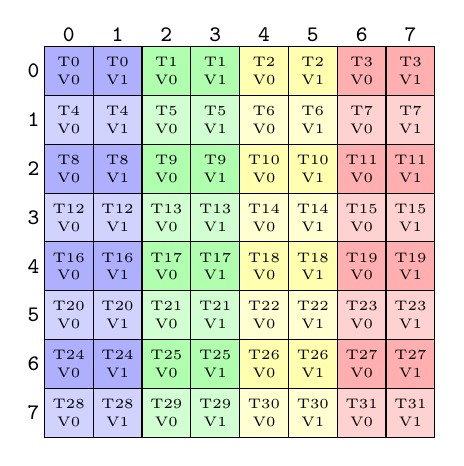
\begin{tikzpicture}[x={(0cm,-0.62cm)},y={(0.62cm,0cm)},every node/.style={minimum size=0.62cm, outer sep=0pt, inner sep=0pt, font=\tiny}]
\node[fill={rgb,255:red,175;green,175;blue,255}] at (0,0) {\shortstack{T0\\V0}};
\node[fill={rgb,255:red,175;green,175;blue,255}] at (0,1) {\shortstack{T0\\V1}};
\node[fill={rgb,255:red,175;green,255;blue,175}] at (0,2) {\shortstack{T1\\V0}};
\node[fill={rgb,255:red,175;green,255;blue,175}] at (0,3) {\shortstack{T1\\V1}};
\node[fill={rgb,255:red,255;green,255;blue,175}] at (0,4) {\shortstack{T2\\V0}};
\node[fill={rgb,255:red,255;green,255;blue,175}] at (0,5) {\shortstack{T2\\V1}};
\node[fill={rgb,255:red,255;green,175;blue,175}] at (0,6) {\shortstack{T3\\V0}};
\node[fill={rgb,255:red,255;green,175;blue,175}] at (0,7) {\shortstack{T3\\V1}};
\node[fill={rgb,255:red,210;green,210;blue,255}] at (1,0) {\shortstack{T4\\V0}};
\node[fill={rgb,255:red,210;green,210;blue,255}] at (1,1) {\shortstack{T4\\V1}};
\node[fill={rgb,255:red,210;green,255;blue,210}] at (1,2) {\shortstack{T5\\V0}};
\node[fill={rgb,255:red,210;green,255;blue,210}] at (1,3) {\shortstack{T5\\V1}};
\node[fill={rgb,255:red,255;green,255;blue,210}] at (1,4) {\shortstack{T6\\V0}};
\node[fill={rgb,255:red,255;green,255;blue,210}] at (1,5) {\shortstack{T6\\V1}};
\node[fill={rgb,255:red,255;green,210;blue,210}] at (1,6) {\shortstack{T7\\V0}};
\node[fill={rgb,255:red,255;green,210;blue,210}] at (1,7) {\shortstack{T7\\V1}};
\node[fill={rgb,255:red,175;green,175;blue,255}] at (2,0) {\shortstack{T8\\V0}};
\node[fill={rgb,255:red,175;green,175;blue,255}] at (2,1) {\shortstack{T8\\V1}};
\node[fill={rgb,255:red,175;green,255;blue,175}] at (2,2) {\shortstack{T9\\V0}};
\node[fill={rgb,255:red,175;green,255;blue,175}] at (2,3) {\shortstack{T9\\V1}};
\node[fill={rgb,255:red,255;green,255;blue,175}] at (2,4) {\shortstack{T10\\V0}};
\node[fill={rgb,255:red,255;green,255;blue,175}] at (2,5) {\shortstack{T10\\V1}};
\node[fill={rgb,255:red,255;green,175;blue,175}] at (2,6) {\shortstack{T11\\V0}};
\node[fill={rgb,255:red,255;green,175;blue,175}] at (2,7) {\shortstack{T11\\V1}};
\node[fill={rgb,255:red,210;green,210;blue,255}] at (3,0) {\shortstack{T12\\V0}};
\node[fill={rgb,255:red,210;green,210;blue,255}] at (3,1) {\shortstack{T12\\V1}};
\node[fill={rgb,255:red,210;green,255;blue,210}] at (3,2) {\shortstack{T13\\V0}};
\node[fill={rgb,255:red,210;green,255;blue,210}] at (3,3) {\shortstack{T13\\V1}};
\node[fill={rgb,255:red,255;green,255;blue,210}] at (3,4) {\shortstack{T14\\V0}};
\node[fill={rgb,255:red,255;green,255;blue,210}] at (3,5) {\shortstack{T14\\V1}};
\node[fill={rgb,255:red,255;green,210;blue,210}] at (3,6) {\shortstack{T15\\V0}};
\node[fill={rgb,255:red,255;green,210;blue,210}] at (3,7) {\shortstack{T15\\V1}};
\node[fill={rgb,255:red,175;green,175;blue,255}] at (4,0) {\shortstack{T16\\V0}};
\node[fill={rgb,255:red,175;green,175;blue,255}] at (4,1) {\shortstack{T16\\V1}};
\node[fill={rgb,255:red,175;green,255;blue,175}] at (4,2) {\shortstack{T17\\V0}};
\node[fill={rgb,255:red,175;green,255;blue,175}] at (4,3) {\shortstack{T17\\V1}};
\node[fill={rgb,255:red,255;green,255;blue,175}] at (4,4) {\shortstack{T18\\V0}};
\node[fill={rgb,255:red,255;green,255;blue,175}] at (4,5) {\shortstack{T18\\V1}};
\node[fill={rgb,255:red,255;green,175;blue,175}] at (4,6) {\shortstack{T19\\V0}};
\node[fill={rgb,255:red,255;green,175;blue,175}] at (4,7) {\shortstack{T19\\V1}};
\node[fill={rgb,255:red,210;green,210;blue,255}] at (5,0) {\shortstack{T20\\V0}};
\node[fill={rgb,255:red,210;green,210;blue,255}] at (5,1) {\shortstack{T20\\V1}};
\node[fill={rgb,255:red,210;green,255;blue,210}] at (5,2) {\shortstack{T21\\V0}};
\node[fill={rgb,255:red,210;green,255;blue,210}] at (5,3) {\shortstack{T21\\V1}};
\node[fill={rgb,255:red,255;green,255;blue,210}] at (5,4) {\shortstack{T22\\V0}};
\node[fill={rgb,255:red,255;green,255;blue,210}] at (5,5) {\shortstack{T22\\V1}};
\node[fill={rgb,255:red,255;green,210;blue,210}] at (5,6) {\shortstack{T23\\V0}};
\node[fill={rgb,255:red,255;green,210;blue,210}] at (5,7) {\shortstack{T23\\V1}};
\node[fill={rgb,255:red,175;green,175;blue,255}] at (6,0) {\shortstack{T24\\V0}};
\node[fill={rgb,255:red,175;green,175;blue,255}] at (6,1) {\shortstack{T24\\V1}};
\node[fill={rgb,255:red,175;green,255;blue,175}] at (6,2) {\shortstack{T25\\V0}};
\node[fill={rgb,255:red,175;green,255;blue,175}] at (6,3) {\shortstack{T25\\V1}};
\node[fill={rgb,255:red,255;green,255;blue,175}] at (6,4) {\shortstack{T26\\V0}};
\node[fill={rgb,255:red,255;green,255;blue,175}] at (6,5) {\shortstack{T26\\V1}};
\node[fill={rgb,255:red,255;green,175;blue,175}] at (6,6) {\shortstack{T27\\V0}};
\node[fill={rgb,255:red,255;green,175;blue,175}] at (6,7) {\shortstack{T27\\V1}};
\node[fill={rgb,255:red,210;green,210;blue,255}] at (7,0) {\shortstack{T28\\V0}};
\node[fill={rgb,255:red,210;green,210;blue,255}] at (7,1) {\shortstack{T28\\V1}};
\node[fill={rgb,255:red,210;green,255;blue,210}] at (7,2) {\shortstack{T29\\V0}};
\node[fill={rgb,255:red,210;green,255;blue,210}] at (7,3) {\shortstack{T29\\V1}};
\node[fill={rgb,255:red,255;green,255;blue,210}] at (7,4) {\shortstack{T30\\V0}};
\node[fill={rgb,255:red,255;green,255;blue,210}] at (7,5) {\shortstack{T30\\V1}};
\node[fill={rgb,255:red,255;green,210;blue,210}] at (7,6) {\shortstack{T31\\V0}};
\node[fill={rgb,255:red,255;green,210;blue,210}] at (7,7) {\shortstack{T31\\V1}};
\draw[color=black,thin,step=0.62cm,shift={(-0.5,-0.5)}] (0,0) grid (8,8);
\node[anchor=east,minimum size=0pt,font=\footnotesize] at (0,-0.6) {\texttt{0}};
\node[anchor=east,minimum size=0pt,font=\footnotesize] at (1,-0.6) {\texttt{1}};
\node[anchor=east,minimum size=0pt,font=\footnotesize] at (2,-0.6) {\texttt{2}};
\node[anchor=east,minimum size=0pt,font=\footnotesize] at (3,-0.6) {\texttt{3}};
\node[anchor=east,minimum size=0pt,font=\footnotesize] at (4,-0.6) {\texttt{4}};
\node[anchor=east,minimum size=0pt,font=\footnotesize] at (5,-0.6) {\texttt{5}};
\node[anchor=east,minimum size=0pt,font=\footnotesize] at (6,-0.6) {\texttt{6}};
\node[anchor=east,minimum size=0pt,font=\footnotesize] at (7,-0.6) {\texttt{7}};
\node[minimum size=0pt,font=\footnotesize] at (-0.75,0) {\texttt{0}};
\node[minimum size=0pt,font=\footnotesize] at (-0.75,1) {\texttt{1}};
\node[minimum size=0pt,font=\footnotesize] at (-0.75,2) {\texttt{2}};
\node[minimum size=0pt,font=\footnotesize] at (-0.75,3) {\texttt{3}};
\node[minimum size=0pt,font=\footnotesize] at (-0.75,4) {\texttt{4}};
\node[minimum size=0pt,font=\footnotesize] at (-0.75,5) {\texttt{5}};
\node[minimum size=0pt,font=\footnotesize] at (-0.75,6) {\texttt{6}};
\node[minimum size=0pt,font=\footnotesize] at (-0.75,7) {\texttt{7}};
\end{tikzpicture}
\end{minipage}
\end{center}

A kernel uses them through the operations. Two warps, $W = 2{:}1$, computing
a $16 \times 16$ tile side by side have the thread-value map
\[
\divideop\big(\mathrm{canonical}((16,16)),\ (16,8)\big) \circ \interleave(F_C, W),
\]
with domain $(\text{warp}, (\text{lane}, \text{value}))$, and one warp loading
the four $8 \times 8$ matrices of an $8 \times 32$ tile with
\texttt{ldmatrix.x4} has
\[
\divideop\big(\mathrm{canonical}((8,32)),\ (8,8)\big) \circ \interleave(F_{\mathrm{ld}}, 4{:}1),
\]
with domain $(\text{matrix}, (\text{lane}, \text{value}))$. Coloured by warp
and by matrix respectively; in the first, cells are labelled by the thread
$32w + \text{lane}$:
\begin{center}
two warps on $16 \times 16$\\[4pt]
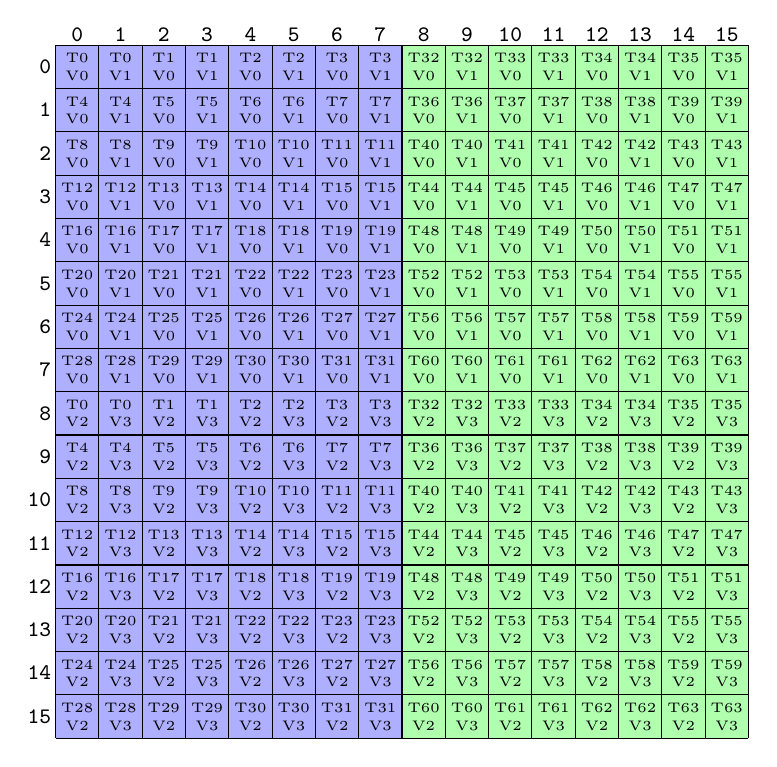
\begin{tikzpicture}[x={(0cm,-0.55cm)},y={(0.55cm,0cm)},every node/.style={minimum size=0.55cm, outer sep=0pt, inner sep=0pt, font=\tiny}]
\node[fill={rgb,255:red,175;green,175;blue,255}] at (0,0) {\shortstack{T0\\V0}};
\node[fill={rgb,255:red,175;green,175;blue,255}] at (0,1) {\shortstack{T0\\V1}};
\node[fill={rgb,255:red,175;green,175;blue,255}] at (0,2) {\shortstack{T1\\V0}};
\node[fill={rgb,255:red,175;green,175;blue,255}] at (0,3) {\shortstack{T1\\V1}};
\node[fill={rgb,255:red,175;green,175;blue,255}] at (0,4) {\shortstack{T2\\V0}};
\node[fill={rgb,255:red,175;green,175;blue,255}] at (0,5) {\shortstack{T2\\V1}};
\node[fill={rgb,255:red,175;green,175;blue,255}] at (0,6) {\shortstack{T3\\V0}};
\node[fill={rgb,255:red,175;green,175;blue,255}] at (0,7) {\shortstack{T3\\V1}};
\node[fill={rgb,255:red,175;green,255;blue,175}] at (0,8) {\shortstack{T32\\V0}};
\node[fill={rgb,255:red,175;green,255;blue,175}] at (0,9) {\shortstack{T32\\V1}};
\node[fill={rgb,255:red,175;green,255;blue,175}] at (0,10) {\shortstack{T33\\V0}};
\node[fill={rgb,255:red,175;green,255;blue,175}] at (0,11) {\shortstack{T33\\V1}};
\node[fill={rgb,255:red,175;green,255;blue,175}] at (0,12) {\shortstack{T34\\V0}};
\node[fill={rgb,255:red,175;green,255;blue,175}] at (0,13) {\shortstack{T34\\V1}};
\node[fill={rgb,255:red,175;green,255;blue,175}] at (0,14) {\shortstack{T35\\V0}};
\node[fill={rgb,255:red,175;green,255;blue,175}] at (0,15) {\shortstack{T35\\V1}};
\node[fill={rgb,255:red,175;green,175;blue,255}] at (1,0) {\shortstack{T4\\V0}};
\node[fill={rgb,255:red,175;green,175;blue,255}] at (1,1) {\shortstack{T4\\V1}};
\node[fill={rgb,255:red,175;green,175;blue,255}] at (1,2) {\shortstack{T5\\V0}};
\node[fill={rgb,255:red,175;green,175;blue,255}] at (1,3) {\shortstack{T5\\V1}};
\node[fill={rgb,255:red,175;green,175;blue,255}] at (1,4) {\shortstack{T6\\V0}};
\node[fill={rgb,255:red,175;green,175;blue,255}] at (1,5) {\shortstack{T6\\V1}};
\node[fill={rgb,255:red,175;green,175;blue,255}] at (1,6) {\shortstack{T7\\V0}};
\node[fill={rgb,255:red,175;green,175;blue,255}] at (1,7) {\shortstack{T7\\V1}};
\node[fill={rgb,255:red,175;green,255;blue,175}] at (1,8) {\shortstack{T36\\V0}};
\node[fill={rgb,255:red,175;green,255;blue,175}] at (1,9) {\shortstack{T36\\V1}};
\node[fill={rgb,255:red,175;green,255;blue,175}] at (1,10) {\shortstack{T37\\V0}};
\node[fill={rgb,255:red,175;green,255;blue,175}] at (1,11) {\shortstack{T37\\V1}};
\node[fill={rgb,255:red,175;green,255;blue,175}] at (1,12) {\shortstack{T38\\V0}};
\node[fill={rgb,255:red,175;green,255;blue,175}] at (1,13) {\shortstack{T38\\V1}};
\node[fill={rgb,255:red,175;green,255;blue,175}] at (1,14) {\shortstack{T39\\V0}};
\node[fill={rgb,255:red,175;green,255;blue,175}] at (1,15) {\shortstack{T39\\V1}};
\node[fill={rgb,255:red,175;green,175;blue,255}] at (2,0) {\shortstack{T8\\V0}};
\node[fill={rgb,255:red,175;green,175;blue,255}] at (2,1) {\shortstack{T8\\V1}};
\node[fill={rgb,255:red,175;green,175;blue,255}] at (2,2) {\shortstack{T9\\V0}};
\node[fill={rgb,255:red,175;green,175;blue,255}] at (2,3) {\shortstack{T9\\V1}};
\node[fill={rgb,255:red,175;green,175;blue,255}] at (2,4) {\shortstack{T10\\V0}};
\node[fill={rgb,255:red,175;green,175;blue,255}] at (2,5) {\shortstack{T10\\V1}};
\node[fill={rgb,255:red,175;green,175;blue,255}] at (2,6) {\shortstack{T11\\V0}};
\node[fill={rgb,255:red,175;green,175;blue,255}] at (2,7) {\shortstack{T11\\V1}};
\node[fill={rgb,255:red,175;green,255;blue,175}] at (2,8) {\shortstack{T40\\V0}};
\node[fill={rgb,255:red,175;green,255;blue,175}] at (2,9) {\shortstack{T40\\V1}};
\node[fill={rgb,255:red,175;green,255;blue,175}] at (2,10) {\shortstack{T41\\V0}};
\node[fill={rgb,255:red,175;green,255;blue,175}] at (2,11) {\shortstack{T41\\V1}};
\node[fill={rgb,255:red,175;green,255;blue,175}] at (2,12) {\shortstack{T42\\V0}};
\node[fill={rgb,255:red,175;green,255;blue,175}] at (2,13) {\shortstack{T42\\V1}};
\node[fill={rgb,255:red,175;green,255;blue,175}] at (2,14) {\shortstack{T43\\V0}};
\node[fill={rgb,255:red,175;green,255;blue,175}] at (2,15) {\shortstack{T43\\V1}};
\node[fill={rgb,255:red,175;green,175;blue,255}] at (3,0) {\shortstack{T12\\V0}};
\node[fill={rgb,255:red,175;green,175;blue,255}] at (3,1) {\shortstack{T12\\V1}};
\node[fill={rgb,255:red,175;green,175;blue,255}] at (3,2) {\shortstack{T13\\V0}};
\node[fill={rgb,255:red,175;green,175;blue,255}] at (3,3) {\shortstack{T13\\V1}};
\node[fill={rgb,255:red,175;green,175;blue,255}] at (3,4) {\shortstack{T14\\V0}};
\node[fill={rgb,255:red,175;green,175;blue,255}] at (3,5) {\shortstack{T14\\V1}};
\node[fill={rgb,255:red,175;green,175;blue,255}] at (3,6) {\shortstack{T15\\V0}};
\node[fill={rgb,255:red,175;green,175;blue,255}] at (3,7) {\shortstack{T15\\V1}};
\node[fill={rgb,255:red,175;green,255;blue,175}] at (3,8) {\shortstack{T44\\V0}};
\node[fill={rgb,255:red,175;green,255;blue,175}] at (3,9) {\shortstack{T44\\V1}};
\node[fill={rgb,255:red,175;green,255;blue,175}] at (3,10) {\shortstack{T45\\V0}};
\node[fill={rgb,255:red,175;green,255;blue,175}] at (3,11) {\shortstack{T45\\V1}};
\node[fill={rgb,255:red,175;green,255;blue,175}] at (3,12) {\shortstack{T46\\V0}};
\node[fill={rgb,255:red,175;green,255;blue,175}] at (3,13) {\shortstack{T46\\V1}};
\node[fill={rgb,255:red,175;green,255;blue,175}] at (3,14) {\shortstack{T47\\V0}};
\node[fill={rgb,255:red,175;green,255;blue,175}] at (3,15) {\shortstack{T47\\V1}};
\node[fill={rgb,255:red,175;green,175;blue,255}] at (4,0) {\shortstack{T16\\V0}};
\node[fill={rgb,255:red,175;green,175;blue,255}] at (4,1) {\shortstack{T16\\V1}};
\node[fill={rgb,255:red,175;green,175;blue,255}] at (4,2) {\shortstack{T17\\V0}};
\node[fill={rgb,255:red,175;green,175;blue,255}] at (4,3) {\shortstack{T17\\V1}};
\node[fill={rgb,255:red,175;green,175;blue,255}] at (4,4) {\shortstack{T18\\V0}};
\node[fill={rgb,255:red,175;green,175;blue,255}] at (4,5) {\shortstack{T18\\V1}};
\node[fill={rgb,255:red,175;green,175;blue,255}] at (4,6) {\shortstack{T19\\V0}};
\node[fill={rgb,255:red,175;green,175;blue,255}] at (4,7) {\shortstack{T19\\V1}};
\node[fill={rgb,255:red,175;green,255;blue,175}] at (4,8) {\shortstack{T48\\V0}};
\node[fill={rgb,255:red,175;green,255;blue,175}] at (4,9) {\shortstack{T48\\V1}};
\node[fill={rgb,255:red,175;green,255;blue,175}] at (4,10) {\shortstack{T49\\V0}};
\node[fill={rgb,255:red,175;green,255;blue,175}] at (4,11) {\shortstack{T49\\V1}};
\node[fill={rgb,255:red,175;green,255;blue,175}] at (4,12) {\shortstack{T50\\V0}};
\node[fill={rgb,255:red,175;green,255;blue,175}] at (4,13) {\shortstack{T50\\V1}};
\node[fill={rgb,255:red,175;green,255;blue,175}] at (4,14) {\shortstack{T51\\V0}};
\node[fill={rgb,255:red,175;green,255;blue,175}] at (4,15) {\shortstack{T51\\V1}};
\node[fill={rgb,255:red,175;green,175;blue,255}] at (5,0) {\shortstack{T20\\V0}};
\node[fill={rgb,255:red,175;green,175;blue,255}] at (5,1) {\shortstack{T20\\V1}};
\node[fill={rgb,255:red,175;green,175;blue,255}] at (5,2) {\shortstack{T21\\V0}};
\node[fill={rgb,255:red,175;green,175;blue,255}] at (5,3) {\shortstack{T21\\V1}};
\node[fill={rgb,255:red,175;green,175;blue,255}] at (5,4) {\shortstack{T22\\V0}};
\node[fill={rgb,255:red,175;green,175;blue,255}] at (5,5) {\shortstack{T22\\V1}};
\node[fill={rgb,255:red,175;green,175;blue,255}] at (5,6) {\shortstack{T23\\V0}};
\node[fill={rgb,255:red,175;green,175;blue,255}] at (5,7) {\shortstack{T23\\V1}};
\node[fill={rgb,255:red,175;green,255;blue,175}] at (5,8) {\shortstack{T52\\V0}};
\node[fill={rgb,255:red,175;green,255;blue,175}] at (5,9) {\shortstack{T52\\V1}};
\node[fill={rgb,255:red,175;green,255;blue,175}] at (5,10) {\shortstack{T53\\V0}};
\node[fill={rgb,255:red,175;green,255;blue,175}] at (5,11) {\shortstack{T53\\V1}};
\node[fill={rgb,255:red,175;green,255;blue,175}] at (5,12) {\shortstack{T54\\V0}};
\node[fill={rgb,255:red,175;green,255;blue,175}] at (5,13) {\shortstack{T54\\V1}};
\node[fill={rgb,255:red,175;green,255;blue,175}] at (5,14) {\shortstack{T55\\V0}};
\node[fill={rgb,255:red,175;green,255;blue,175}] at (5,15) {\shortstack{T55\\V1}};
\node[fill={rgb,255:red,175;green,175;blue,255}] at (6,0) {\shortstack{T24\\V0}};
\node[fill={rgb,255:red,175;green,175;blue,255}] at (6,1) {\shortstack{T24\\V1}};
\node[fill={rgb,255:red,175;green,175;blue,255}] at (6,2) {\shortstack{T25\\V0}};
\node[fill={rgb,255:red,175;green,175;blue,255}] at (6,3) {\shortstack{T25\\V1}};
\node[fill={rgb,255:red,175;green,175;blue,255}] at (6,4) {\shortstack{T26\\V0}};
\node[fill={rgb,255:red,175;green,175;blue,255}] at (6,5) {\shortstack{T26\\V1}};
\node[fill={rgb,255:red,175;green,175;blue,255}] at (6,6) {\shortstack{T27\\V0}};
\node[fill={rgb,255:red,175;green,175;blue,255}] at (6,7) {\shortstack{T27\\V1}};
\node[fill={rgb,255:red,175;green,255;blue,175}] at (6,8) {\shortstack{T56\\V0}};
\node[fill={rgb,255:red,175;green,255;blue,175}] at (6,9) {\shortstack{T56\\V1}};
\node[fill={rgb,255:red,175;green,255;blue,175}] at (6,10) {\shortstack{T57\\V0}};
\node[fill={rgb,255:red,175;green,255;blue,175}] at (6,11) {\shortstack{T57\\V1}};
\node[fill={rgb,255:red,175;green,255;blue,175}] at (6,12) {\shortstack{T58\\V0}};
\node[fill={rgb,255:red,175;green,255;blue,175}] at (6,13) {\shortstack{T58\\V1}};
\node[fill={rgb,255:red,175;green,255;blue,175}] at (6,14) {\shortstack{T59\\V0}};
\node[fill={rgb,255:red,175;green,255;blue,175}] at (6,15) {\shortstack{T59\\V1}};
\node[fill={rgb,255:red,175;green,175;blue,255}] at (7,0) {\shortstack{T28\\V0}};
\node[fill={rgb,255:red,175;green,175;blue,255}] at (7,1) {\shortstack{T28\\V1}};
\node[fill={rgb,255:red,175;green,175;blue,255}] at (7,2) {\shortstack{T29\\V0}};
\node[fill={rgb,255:red,175;green,175;blue,255}] at (7,3) {\shortstack{T29\\V1}};
\node[fill={rgb,255:red,175;green,175;blue,255}] at (7,4) {\shortstack{T30\\V0}};
\node[fill={rgb,255:red,175;green,175;blue,255}] at (7,5) {\shortstack{T30\\V1}};
\node[fill={rgb,255:red,175;green,175;blue,255}] at (7,6) {\shortstack{T31\\V0}};
\node[fill={rgb,255:red,175;green,175;blue,255}] at (7,7) {\shortstack{T31\\V1}};
\node[fill={rgb,255:red,175;green,255;blue,175}] at (7,8) {\shortstack{T60\\V0}};
\node[fill={rgb,255:red,175;green,255;blue,175}] at (7,9) {\shortstack{T60\\V1}};
\node[fill={rgb,255:red,175;green,255;blue,175}] at (7,10) {\shortstack{T61\\V0}};
\node[fill={rgb,255:red,175;green,255;blue,175}] at (7,11) {\shortstack{T61\\V1}};
\node[fill={rgb,255:red,175;green,255;blue,175}] at (7,12) {\shortstack{T62\\V0}};
\node[fill={rgb,255:red,175;green,255;blue,175}] at (7,13) {\shortstack{T62\\V1}};
\node[fill={rgb,255:red,175;green,255;blue,175}] at (7,14) {\shortstack{T63\\V0}};
\node[fill={rgb,255:red,175;green,255;blue,175}] at (7,15) {\shortstack{T63\\V1}};
\node[fill={rgb,255:red,175;green,175;blue,255}] at (8,0) {\shortstack{T0\\V2}};
\node[fill={rgb,255:red,175;green,175;blue,255}] at (8,1) {\shortstack{T0\\V3}};
\node[fill={rgb,255:red,175;green,175;blue,255}] at (8,2) {\shortstack{T1\\V2}};
\node[fill={rgb,255:red,175;green,175;blue,255}] at (8,3) {\shortstack{T1\\V3}};
\node[fill={rgb,255:red,175;green,175;blue,255}] at (8,4) {\shortstack{T2\\V2}};
\node[fill={rgb,255:red,175;green,175;blue,255}] at (8,5) {\shortstack{T2\\V3}};
\node[fill={rgb,255:red,175;green,175;blue,255}] at (8,6) {\shortstack{T3\\V2}};
\node[fill={rgb,255:red,175;green,175;blue,255}] at (8,7) {\shortstack{T3\\V3}};
\node[fill={rgb,255:red,175;green,255;blue,175}] at (8,8) {\shortstack{T32\\V2}};
\node[fill={rgb,255:red,175;green,255;blue,175}] at (8,9) {\shortstack{T32\\V3}};
\node[fill={rgb,255:red,175;green,255;blue,175}] at (8,10) {\shortstack{T33\\V2}};
\node[fill={rgb,255:red,175;green,255;blue,175}] at (8,11) {\shortstack{T33\\V3}};
\node[fill={rgb,255:red,175;green,255;blue,175}] at (8,12) {\shortstack{T34\\V2}};
\node[fill={rgb,255:red,175;green,255;blue,175}] at (8,13) {\shortstack{T34\\V3}};
\node[fill={rgb,255:red,175;green,255;blue,175}] at (8,14) {\shortstack{T35\\V2}};
\node[fill={rgb,255:red,175;green,255;blue,175}] at (8,15) {\shortstack{T35\\V3}};
\node[fill={rgb,255:red,175;green,175;blue,255}] at (9,0) {\shortstack{T4\\V2}};
\node[fill={rgb,255:red,175;green,175;blue,255}] at (9,1) {\shortstack{T4\\V3}};
\node[fill={rgb,255:red,175;green,175;blue,255}] at (9,2) {\shortstack{T5\\V2}};
\node[fill={rgb,255:red,175;green,175;blue,255}] at (9,3) {\shortstack{T5\\V3}};
\node[fill={rgb,255:red,175;green,175;blue,255}] at (9,4) {\shortstack{T6\\V2}};
\node[fill={rgb,255:red,175;green,175;blue,255}] at (9,5) {\shortstack{T6\\V3}};
\node[fill={rgb,255:red,175;green,175;blue,255}] at (9,6) {\shortstack{T7\\V2}};
\node[fill={rgb,255:red,175;green,175;blue,255}] at (9,7) {\shortstack{T7\\V3}};
\node[fill={rgb,255:red,175;green,255;blue,175}] at (9,8) {\shortstack{T36\\V2}};
\node[fill={rgb,255:red,175;green,255;blue,175}] at (9,9) {\shortstack{T36\\V3}};
\node[fill={rgb,255:red,175;green,255;blue,175}] at (9,10) {\shortstack{T37\\V2}};
\node[fill={rgb,255:red,175;green,255;blue,175}] at (9,11) {\shortstack{T37\\V3}};
\node[fill={rgb,255:red,175;green,255;blue,175}] at (9,12) {\shortstack{T38\\V2}};
\node[fill={rgb,255:red,175;green,255;blue,175}] at (9,13) {\shortstack{T38\\V3}};
\node[fill={rgb,255:red,175;green,255;blue,175}] at (9,14) {\shortstack{T39\\V2}};
\node[fill={rgb,255:red,175;green,255;blue,175}] at (9,15) {\shortstack{T39\\V3}};
\node[fill={rgb,255:red,175;green,175;blue,255}] at (10,0) {\shortstack{T8\\V2}};
\node[fill={rgb,255:red,175;green,175;blue,255}] at (10,1) {\shortstack{T8\\V3}};
\node[fill={rgb,255:red,175;green,175;blue,255}] at (10,2) {\shortstack{T9\\V2}};
\node[fill={rgb,255:red,175;green,175;blue,255}] at (10,3) {\shortstack{T9\\V3}};
\node[fill={rgb,255:red,175;green,175;blue,255}] at (10,4) {\shortstack{T10\\V2}};
\node[fill={rgb,255:red,175;green,175;blue,255}] at (10,5) {\shortstack{T10\\V3}};
\node[fill={rgb,255:red,175;green,175;blue,255}] at (10,6) {\shortstack{T11\\V2}};
\node[fill={rgb,255:red,175;green,175;blue,255}] at (10,7) {\shortstack{T11\\V3}};
\node[fill={rgb,255:red,175;green,255;blue,175}] at (10,8) {\shortstack{T40\\V2}};
\node[fill={rgb,255:red,175;green,255;blue,175}] at (10,9) {\shortstack{T40\\V3}};
\node[fill={rgb,255:red,175;green,255;blue,175}] at (10,10) {\shortstack{T41\\V2}};
\node[fill={rgb,255:red,175;green,255;blue,175}] at (10,11) {\shortstack{T41\\V3}};
\node[fill={rgb,255:red,175;green,255;blue,175}] at (10,12) {\shortstack{T42\\V2}};
\node[fill={rgb,255:red,175;green,255;blue,175}] at (10,13) {\shortstack{T42\\V3}};
\node[fill={rgb,255:red,175;green,255;blue,175}] at (10,14) {\shortstack{T43\\V2}};
\node[fill={rgb,255:red,175;green,255;blue,175}] at (10,15) {\shortstack{T43\\V3}};
\node[fill={rgb,255:red,175;green,175;blue,255}] at (11,0) {\shortstack{T12\\V2}};
\node[fill={rgb,255:red,175;green,175;blue,255}] at (11,1) {\shortstack{T12\\V3}};
\node[fill={rgb,255:red,175;green,175;blue,255}] at (11,2) {\shortstack{T13\\V2}};
\node[fill={rgb,255:red,175;green,175;blue,255}] at (11,3) {\shortstack{T13\\V3}};
\node[fill={rgb,255:red,175;green,175;blue,255}] at (11,4) {\shortstack{T14\\V2}};
\node[fill={rgb,255:red,175;green,175;blue,255}] at (11,5) {\shortstack{T14\\V3}};
\node[fill={rgb,255:red,175;green,175;blue,255}] at (11,6) {\shortstack{T15\\V2}};
\node[fill={rgb,255:red,175;green,175;blue,255}] at (11,7) {\shortstack{T15\\V3}};
\node[fill={rgb,255:red,175;green,255;blue,175}] at (11,8) {\shortstack{T44\\V2}};
\node[fill={rgb,255:red,175;green,255;blue,175}] at (11,9) {\shortstack{T44\\V3}};
\node[fill={rgb,255:red,175;green,255;blue,175}] at (11,10) {\shortstack{T45\\V2}};
\node[fill={rgb,255:red,175;green,255;blue,175}] at (11,11) {\shortstack{T45\\V3}};
\node[fill={rgb,255:red,175;green,255;blue,175}] at (11,12) {\shortstack{T46\\V2}};
\node[fill={rgb,255:red,175;green,255;blue,175}] at (11,13) {\shortstack{T46\\V3}};
\node[fill={rgb,255:red,175;green,255;blue,175}] at (11,14) {\shortstack{T47\\V2}};
\node[fill={rgb,255:red,175;green,255;blue,175}] at (11,15) {\shortstack{T47\\V3}};
\node[fill={rgb,255:red,175;green,175;blue,255}] at (12,0) {\shortstack{T16\\V2}};
\node[fill={rgb,255:red,175;green,175;blue,255}] at (12,1) {\shortstack{T16\\V3}};
\node[fill={rgb,255:red,175;green,175;blue,255}] at (12,2) {\shortstack{T17\\V2}};
\node[fill={rgb,255:red,175;green,175;blue,255}] at (12,3) {\shortstack{T17\\V3}};
\node[fill={rgb,255:red,175;green,175;blue,255}] at (12,4) {\shortstack{T18\\V2}};
\node[fill={rgb,255:red,175;green,175;blue,255}] at (12,5) {\shortstack{T18\\V3}};
\node[fill={rgb,255:red,175;green,175;blue,255}] at (12,6) {\shortstack{T19\\V2}};
\node[fill={rgb,255:red,175;green,175;blue,255}] at (12,7) {\shortstack{T19\\V3}};
\node[fill={rgb,255:red,175;green,255;blue,175}] at (12,8) {\shortstack{T48\\V2}};
\node[fill={rgb,255:red,175;green,255;blue,175}] at (12,9) {\shortstack{T48\\V3}};
\node[fill={rgb,255:red,175;green,255;blue,175}] at (12,10) {\shortstack{T49\\V2}};
\node[fill={rgb,255:red,175;green,255;blue,175}] at (12,11) {\shortstack{T49\\V3}};
\node[fill={rgb,255:red,175;green,255;blue,175}] at (12,12) {\shortstack{T50\\V2}};
\node[fill={rgb,255:red,175;green,255;blue,175}] at (12,13) {\shortstack{T50\\V3}};
\node[fill={rgb,255:red,175;green,255;blue,175}] at (12,14) {\shortstack{T51\\V2}};
\node[fill={rgb,255:red,175;green,255;blue,175}] at (12,15) {\shortstack{T51\\V3}};
\node[fill={rgb,255:red,175;green,175;blue,255}] at (13,0) {\shortstack{T20\\V2}};
\node[fill={rgb,255:red,175;green,175;blue,255}] at (13,1) {\shortstack{T20\\V3}};
\node[fill={rgb,255:red,175;green,175;blue,255}] at (13,2) {\shortstack{T21\\V2}};
\node[fill={rgb,255:red,175;green,175;blue,255}] at (13,3) {\shortstack{T21\\V3}};
\node[fill={rgb,255:red,175;green,175;blue,255}] at (13,4) {\shortstack{T22\\V2}};
\node[fill={rgb,255:red,175;green,175;blue,255}] at (13,5) {\shortstack{T22\\V3}};
\node[fill={rgb,255:red,175;green,175;blue,255}] at (13,6) {\shortstack{T23\\V2}};
\node[fill={rgb,255:red,175;green,175;blue,255}] at (13,7) {\shortstack{T23\\V3}};
\node[fill={rgb,255:red,175;green,255;blue,175}] at (13,8) {\shortstack{T52\\V2}};
\node[fill={rgb,255:red,175;green,255;blue,175}] at (13,9) {\shortstack{T52\\V3}};
\node[fill={rgb,255:red,175;green,255;blue,175}] at (13,10) {\shortstack{T53\\V2}};
\node[fill={rgb,255:red,175;green,255;blue,175}] at (13,11) {\shortstack{T53\\V3}};
\node[fill={rgb,255:red,175;green,255;blue,175}] at (13,12) {\shortstack{T54\\V2}};
\node[fill={rgb,255:red,175;green,255;blue,175}] at (13,13) {\shortstack{T54\\V3}};
\node[fill={rgb,255:red,175;green,255;blue,175}] at (13,14) {\shortstack{T55\\V2}};
\node[fill={rgb,255:red,175;green,255;blue,175}] at (13,15) {\shortstack{T55\\V3}};
\node[fill={rgb,255:red,175;green,175;blue,255}] at (14,0) {\shortstack{T24\\V2}};
\node[fill={rgb,255:red,175;green,175;blue,255}] at (14,1) {\shortstack{T24\\V3}};
\node[fill={rgb,255:red,175;green,175;blue,255}] at (14,2) {\shortstack{T25\\V2}};
\node[fill={rgb,255:red,175;green,175;blue,255}] at (14,3) {\shortstack{T25\\V3}};
\node[fill={rgb,255:red,175;green,175;blue,255}] at (14,4) {\shortstack{T26\\V2}};
\node[fill={rgb,255:red,175;green,175;blue,255}] at (14,5) {\shortstack{T26\\V3}};
\node[fill={rgb,255:red,175;green,175;blue,255}] at (14,6) {\shortstack{T27\\V2}};
\node[fill={rgb,255:red,175;green,175;blue,255}] at (14,7) {\shortstack{T27\\V3}};
\node[fill={rgb,255:red,175;green,255;blue,175}] at (14,8) {\shortstack{T56\\V2}};
\node[fill={rgb,255:red,175;green,255;blue,175}] at (14,9) {\shortstack{T56\\V3}};
\node[fill={rgb,255:red,175;green,255;blue,175}] at (14,10) {\shortstack{T57\\V2}};
\node[fill={rgb,255:red,175;green,255;blue,175}] at (14,11) {\shortstack{T57\\V3}};
\node[fill={rgb,255:red,175;green,255;blue,175}] at (14,12) {\shortstack{T58\\V2}};
\node[fill={rgb,255:red,175;green,255;blue,175}] at (14,13) {\shortstack{T58\\V3}};
\node[fill={rgb,255:red,175;green,255;blue,175}] at (14,14) {\shortstack{T59\\V2}};
\node[fill={rgb,255:red,175;green,255;blue,175}] at (14,15) {\shortstack{T59\\V3}};
\node[fill={rgb,255:red,175;green,175;blue,255}] at (15,0) {\shortstack{T28\\V2}};
\node[fill={rgb,255:red,175;green,175;blue,255}] at (15,1) {\shortstack{T28\\V3}};
\node[fill={rgb,255:red,175;green,175;blue,255}] at (15,2) {\shortstack{T29\\V2}};
\node[fill={rgb,255:red,175;green,175;blue,255}] at (15,3) {\shortstack{T29\\V3}};
\node[fill={rgb,255:red,175;green,175;blue,255}] at (15,4) {\shortstack{T30\\V2}};
\node[fill={rgb,255:red,175;green,175;blue,255}] at (15,5) {\shortstack{T30\\V3}};
\node[fill={rgb,255:red,175;green,175;blue,255}] at (15,6) {\shortstack{T31\\V2}};
\node[fill={rgb,255:red,175;green,175;blue,255}] at (15,7) {\shortstack{T31\\V3}};
\node[fill={rgb,255:red,175;green,255;blue,175}] at (15,8) {\shortstack{T60\\V2}};
\node[fill={rgb,255:red,175;green,255;blue,175}] at (15,9) {\shortstack{T60\\V3}};
\node[fill={rgb,255:red,175;green,255;blue,175}] at (15,10) {\shortstack{T61\\V2}};
\node[fill={rgb,255:red,175;green,255;blue,175}] at (15,11) {\shortstack{T61\\V3}};
\node[fill={rgb,255:red,175;green,255;blue,175}] at (15,12) {\shortstack{T62\\V2}};
\node[fill={rgb,255:red,175;green,255;blue,175}] at (15,13) {\shortstack{T62\\V3}};
\node[fill={rgb,255:red,175;green,255;blue,175}] at (15,14) {\shortstack{T63\\V2}};
\node[fill={rgb,255:red,175;green,255;blue,175}] at (15,15) {\shortstack{T63\\V3}};
\draw[color=black,thin,step=0.55cm,shift={(-0.5,-0.5)}] (0,0) grid (16,16);
\node[anchor=east,minimum size=0pt,font=\footnotesize] at (0,-0.6) {\texttt{0}};
\node[anchor=east,minimum size=0pt,font=\footnotesize] at (1,-0.6) {\texttt{1}};
\node[anchor=east,minimum size=0pt,font=\footnotesize] at (2,-0.6) {\texttt{2}};
\node[anchor=east,minimum size=0pt,font=\footnotesize] at (3,-0.6) {\texttt{3}};
\node[anchor=east,minimum size=0pt,font=\footnotesize] at (4,-0.6) {\texttt{4}};
\node[anchor=east,minimum size=0pt,font=\footnotesize] at (5,-0.6) {\texttt{5}};
\node[anchor=east,minimum size=0pt,font=\footnotesize] at (6,-0.6) {\texttt{6}};
\node[anchor=east,minimum size=0pt,font=\footnotesize] at (7,-0.6) {\texttt{7}};
\node[anchor=east,minimum size=0pt,font=\footnotesize] at (8,-0.6) {\texttt{8}};
\node[anchor=east,minimum size=0pt,font=\footnotesize] at (9,-0.6) {\texttt{9}};
\node[anchor=east,minimum size=0pt,font=\footnotesize] at (10,-0.6) {\texttt{10}};
\node[anchor=east,minimum size=0pt,font=\footnotesize] at (11,-0.6) {\texttt{11}};
\node[anchor=east,minimum size=0pt,font=\footnotesize] at (12,-0.6) {\texttt{12}};
\node[anchor=east,minimum size=0pt,font=\footnotesize] at (13,-0.6) {\texttt{13}};
\node[anchor=east,minimum size=0pt,font=\footnotesize] at (14,-0.6) {\texttt{14}};
\node[anchor=east,minimum size=0pt,font=\footnotesize] at (15,-0.6) {\texttt{15}};
\node[minimum size=0pt,font=\footnotesize] at (-0.75,0) {\texttt{0}};
\node[minimum size=0pt,font=\footnotesize] at (-0.75,1) {\texttt{1}};
\node[minimum size=0pt,font=\footnotesize] at (-0.75,2) {\texttt{2}};
\node[minimum size=0pt,font=\footnotesize] at (-0.75,3) {\texttt{3}};
\node[minimum size=0pt,font=\footnotesize] at (-0.75,4) {\texttt{4}};
\node[minimum size=0pt,font=\footnotesize] at (-0.75,5) {\texttt{5}};
\node[minimum size=0pt,font=\footnotesize] at (-0.75,6) {\texttt{6}};
\node[minimum size=0pt,font=\footnotesize] at (-0.75,7) {\texttt{7}};
\node[minimum size=0pt,font=\footnotesize] at (-0.75,8) {\texttt{8}};
\node[minimum size=0pt,font=\footnotesize] at (-0.75,9) {\texttt{9}};
\node[minimum size=0pt,font=\footnotesize] at (-0.75,10) {\texttt{10}};
\node[minimum size=0pt,font=\footnotesize] at (-0.75,11) {\texttt{11}};
\node[minimum size=0pt,font=\footnotesize] at (-0.75,12) {\texttt{12}};
\node[minimum size=0pt,font=\footnotesize] at (-0.75,13) {\texttt{13}};
\node[minimum size=0pt,font=\footnotesize] at (-0.75,14) {\texttt{14}};
\node[minimum size=0pt,font=\footnotesize] at (-0.75,15) {\texttt{15}};
\end{tikzpicture}
\end{center}

\begin{center}
\texttt{ldmatrix.x4} on $8 \times 32$\\[4pt]
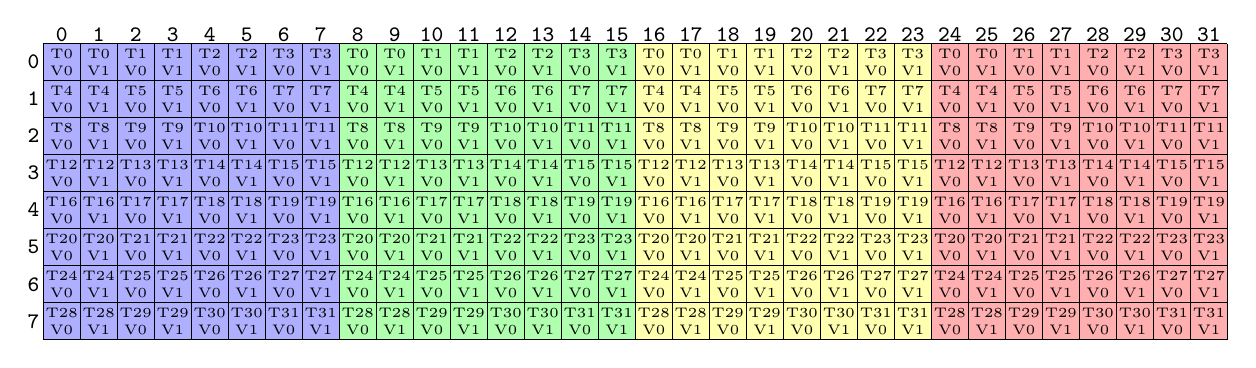
\begin{tikzpicture}[x={(0cm,-0.47cm)},y={(0.47cm,0cm)},every node/.style={minimum size=0.47cm, outer sep=0pt, inner sep=0pt, font=\tiny}]
\node[fill={rgb,255:red,175;green,175;blue,255}] at (0,0) {\shortstack{T0\\V0}};
\node[fill={rgb,255:red,175;green,175;blue,255}] at (0,1) {\shortstack{T0\\V1}};
\node[fill={rgb,255:red,175;green,175;blue,255}] at (0,2) {\shortstack{T1\\V0}};
\node[fill={rgb,255:red,175;green,175;blue,255}] at (0,3) {\shortstack{T1\\V1}};
\node[fill={rgb,255:red,175;green,175;blue,255}] at (0,4) {\shortstack{T2\\V0}};
\node[fill={rgb,255:red,175;green,175;blue,255}] at (0,5) {\shortstack{T2\\V1}};
\node[fill={rgb,255:red,175;green,175;blue,255}] at (0,6) {\shortstack{T3\\V0}};
\node[fill={rgb,255:red,175;green,175;blue,255}] at (0,7) {\shortstack{T3\\V1}};
\node[fill={rgb,255:red,175;green,255;blue,175}] at (0,8) {\shortstack{T0\\V0}};
\node[fill={rgb,255:red,175;green,255;blue,175}] at (0,9) {\shortstack{T0\\V1}};
\node[fill={rgb,255:red,175;green,255;blue,175}] at (0,10) {\shortstack{T1\\V0}};
\node[fill={rgb,255:red,175;green,255;blue,175}] at (0,11) {\shortstack{T1\\V1}};
\node[fill={rgb,255:red,175;green,255;blue,175}] at (0,12) {\shortstack{T2\\V0}};
\node[fill={rgb,255:red,175;green,255;blue,175}] at (0,13) {\shortstack{T2\\V1}};
\node[fill={rgb,255:red,175;green,255;blue,175}] at (0,14) {\shortstack{T3\\V0}};
\node[fill={rgb,255:red,175;green,255;blue,175}] at (0,15) {\shortstack{T3\\V1}};
\node[fill={rgb,255:red,255;green,255;blue,175}] at (0,16) {\shortstack{T0\\V0}};
\node[fill={rgb,255:red,255;green,255;blue,175}] at (0,17) {\shortstack{T0\\V1}};
\node[fill={rgb,255:red,255;green,255;blue,175}] at (0,18) {\shortstack{T1\\V0}};
\node[fill={rgb,255:red,255;green,255;blue,175}] at (0,19) {\shortstack{T1\\V1}};
\node[fill={rgb,255:red,255;green,255;blue,175}] at (0,20) {\shortstack{T2\\V0}};
\node[fill={rgb,255:red,255;green,255;blue,175}] at (0,21) {\shortstack{T2\\V1}};
\node[fill={rgb,255:red,255;green,255;blue,175}] at (0,22) {\shortstack{T3\\V0}};
\node[fill={rgb,255:red,255;green,255;blue,175}] at (0,23) {\shortstack{T3\\V1}};
\node[fill={rgb,255:red,255;green,175;blue,175}] at (0,24) {\shortstack{T0\\V0}};
\node[fill={rgb,255:red,255;green,175;blue,175}] at (0,25) {\shortstack{T0\\V1}};
\node[fill={rgb,255:red,255;green,175;blue,175}] at (0,26) {\shortstack{T1\\V0}};
\node[fill={rgb,255:red,255;green,175;blue,175}] at (0,27) {\shortstack{T1\\V1}};
\node[fill={rgb,255:red,255;green,175;blue,175}] at (0,28) {\shortstack{T2\\V0}};
\node[fill={rgb,255:red,255;green,175;blue,175}] at (0,29) {\shortstack{T2\\V1}};
\node[fill={rgb,255:red,255;green,175;blue,175}] at (0,30) {\shortstack{T3\\V0}};
\node[fill={rgb,255:red,255;green,175;blue,175}] at (0,31) {\shortstack{T3\\V1}};
\node[fill={rgb,255:red,175;green,175;blue,255}] at (1,0) {\shortstack{T4\\V0}};
\node[fill={rgb,255:red,175;green,175;blue,255}] at (1,1) {\shortstack{T4\\V1}};
\node[fill={rgb,255:red,175;green,175;blue,255}] at (1,2) {\shortstack{T5\\V0}};
\node[fill={rgb,255:red,175;green,175;blue,255}] at (1,3) {\shortstack{T5\\V1}};
\node[fill={rgb,255:red,175;green,175;blue,255}] at (1,4) {\shortstack{T6\\V0}};
\node[fill={rgb,255:red,175;green,175;blue,255}] at (1,5) {\shortstack{T6\\V1}};
\node[fill={rgb,255:red,175;green,175;blue,255}] at (1,6) {\shortstack{T7\\V0}};
\node[fill={rgb,255:red,175;green,175;blue,255}] at (1,7) {\shortstack{T7\\V1}};
\node[fill={rgb,255:red,175;green,255;blue,175}] at (1,8) {\shortstack{T4\\V0}};
\node[fill={rgb,255:red,175;green,255;blue,175}] at (1,9) {\shortstack{T4\\V1}};
\node[fill={rgb,255:red,175;green,255;blue,175}] at (1,10) {\shortstack{T5\\V0}};
\node[fill={rgb,255:red,175;green,255;blue,175}] at (1,11) {\shortstack{T5\\V1}};
\node[fill={rgb,255:red,175;green,255;blue,175}] at (1,12) {\shortstack{T6\\V0}};
\node[fill={rgb,255:red,175;green,255;blue,175}] at (1,13) {\shortstack{T6\\V1}};
\node[fill={rgb,255:red,175;green,255;blue,175}] at (1,14) {\shortstack{T7\\V0}};
\node[fill={rgb,255:red,175;green,255;blue,175}] at (1,15) {\shortstack{T7\\V1}};
\node[fill={rgb,255:red,255;green,255;blue,175}] at (1,16) {\shortstack{T4\\V0}};
\node[fill={rgb,255:red,255;green,255;blue,175}] at (1,17) {\shortstack{T4\\V1}};
\node[fill={rgb,255:red,255;green,255;blue,175}] at (1,18) {\shortstack{T5\\V0}};
\node[fill={rgb,255:red,255;green,255;blue,175}] at (1,19) {\shortstack{T5\\V1}};
\node[fill={rgb,255:red,255;green,255;blue,175}] at (1,20) {\shortstack{T6\\V0}};
\node[fill={rgb,255:red,255;green,255;blue,175}] at (1,21) {\shortstack{T6\\V1}};
\node[fill={rgb,255:red,255;green,255;blue,175}] at (1,22) {\shortstack{T7\\V0}};
\node[fill={rgb,255:red,255;green,255;blue,175}] at (1,23) {\shortstack{T7\\V1}};
\node[fill={rgb,255:red,255;green,175;blue,175}] at (1,24) {\shortstack{T4\\V0}};
\node[fill={rgb,255:red,255;green,175;blue,175}] at (1,25) {\shortstack{T4\\V1}};
\node[fill={rgb,255:red,255;green,175;blue,175}] at (1,26) {\shortstack{T5\\V0}};
\node[fill={rgb,255:red,255;green,175;blue,175}] at (1,27) {\shortstack{T5\\V1}};
\node[fill={rgb,255:red,255;green,175;blue,175}] at (1,28) {\shortstack{T6\\V0}};
\node[fill={rgb,255:red,255;green,175;blue,175}] at (1,29) {\shortstack{T6\\V1}};
\node[fill={rgb,255:red,255;green,175;blue,175}] at (1,30) {\shortstack{T7\\V0}};
\node[fill={rgb,255:red,255;green,175;blue,175}] at (1,31) {\shortstack{T7\\V1}};
\node[fill={rgb,255:red,175;green,175;blue,255}] at (2,0) {\shortstack{T8\\V0}};
\node[fill={rgb,255:red,175;green,175;blue,255}] at (2,1) {\shortstack{T8\\V1}};
\node[fill={rgb,255:red,175;green,175;blue,255}] at (2,2) {\shortstack{T9\\V0}};
\node[fill={rgb,255:red,175;green,175;blue,255}] at (2,3) {\shortstack{T9\\V1}};
\node[fill={rgb,255:red,175;green,175;blue,255}] at (2,4) {\shortstack{T10\\V0}};
\node[fill={rgb,255:red,175;green,175;blue,255}] at (2,5) {\shortstack{T10\\V1}};
\node[fill={rgb,255:red,175;green,175;blue,255}] at (2,6) {\shortstack{T11\\V0}};
\node[fill={rgb,255:red,175;green,175;blue,255}] at (2,7) {\shortstack{T11\\V1}};
\node[fill={rgb,255:red,175;green,255;blue,175}] at (2,8) {\shortstack{T8\\V0}};
\node[fill={rgb,255:red,175;green,255;blue,175}] at (2,9) {\shortstack{T8\\V1}};
\node[fill={rgb,255:red,175;green,255;blue,175}] at (2,10) {\shortstack{T9\\V0}};
\node[fill={rgb,255:red,175;green,255;blue,175}] at (2,11) {\shortstack{T9\\V1}};
\node[fill={rgb,255:red,175;green,255;blue,175}] at (2,12) {\shortstack{T10\\V0}};
\node[fill={rgb,255:red,175;green,255;blue,175}] at (2,13) {\shortstack{T10\\V1}};
\node[fill={rgb,255:red,175;green,255;blue,175}] at (2,14) {\shortstack{T11\\V0}};
\node[fill={rgb,255:red,175;green,255;blue,175}] at (2,15) {\shortstack{T11\\V1}};
\node[fill={rgb,255:red,255;green,255;blue,175}] at (2,16) {\shortstack{T8\\V0}};
\node[fill={rgb,255:red,255;green,255;blue,175}] at (2,17) {\shortstack{T8\\V1}};
\node[fill={rgb,255:red,255;green,255;blue,175}] at (2,18) {\shortstack{T9\\V0}};
\node[fill={rgb,255:red,255;green,255;blue,175}] at (2,19) {\shortstack{T9\\V1}};
\node[fill={rgb,255:red,255;green,255;blue,175}] at (2,20) {\shortstack{T10\\V0}};
\node[fill={rgb,255:red,255;green,255;blue,175}] at (2,21) {\shortstack{T10\\V1}};
\node[fill={rgb,255:red,255;green,255;blue,175}] at (2,22) {\shortstack{T11\\V0}};
\node[fill={rgb,255:red,255;green,255;blue,175}] at (2,23) {\shortstack{T11\\V1}};
\node[fill={rgb,255:red,255;green,175;blue,175}] at (2,24) {\shortstack{T8\\V0}};
\node[fill={rgb,255:red,255;green,175;blue,175}] at (2,25) {\shortstack{T8\\V1}};
\node[fill={rgb,255:red,255;green,175;blue,175}] at (2,26) {\shortstack{T9\\V0}};
\node[fill={rgb,255:red,255;green,175;blue,175}] at (2,27) {\shortstack{T9\\V1}};
\node[fill={rgb,255:red,255;green,175;blue,175}] at (2,28) {\shortstack{T10\\V0}};
\node[fill={rgb,255:red,255;green,175;blue,175}] at (2,29) {\shortstack{T10\\V1}};
\node[fill={rgb,255:red,255;green,175;blue,175}] at (2,30) {\shortstack{T11\\V0}};
\node[fill={rgb,255:red,255;green,175;blue,175}] at (2,31) {\shortstack{T11\\V1}};
\node[fill={rgb,255:red,175;green,175;blue,255}] at (3,0) {\shortstack{T12\\V0}};
\node[fill={rgb,255:red,175;green,175;blue,255}] at (3,1) {\shortstack{T12\\V1}};
\node[fill={rgb,255:red,175;green,175;blue,255}] at (3,2) {\shortstack{T13\\V0}};
\node[fill={rgb,255:red,175;green,175;blue,255}] at (3,3) {\shortstack{T13\\V1}};
\node[fill={rgb,255:red,175;green,175;blue,255}] at (3,4) {\shortstack{T14\\V0}};
\node[fill={rgb,255:red,175;green,175;blue,255}] at (3,5) {\shortstack{T14\\V1}};
\node[fill={rgb,255:red,175;green,175;blue,255}] at (3,6) {\shortstack{T15\\V0}};
\node[fill={rgb,255:red,175;green,175;blue,255}] at (3,7) {\shortstack{T15\\V1}};
\node[fill={rgb,255:red,175;green,255;blue,175}] at (3,8) {\shortstack{T12\\V0}};
\node[fill={rgb,255:red,175;green,255;blue,175}] at (3,9) {\shortstack{T12\\V1}};
\node[fill={rgb,255:red,175;green,255;blue,175}] at (3,10) {\shortstack{T13\\V0}};
\node[fill={rgb,255:red,175;green,255;blue,175}] at (3,11) {\shortstack{T13\\V1}};
\node[fill={rgb,255:red,175;green,255;blue,175}] at (3,12) {\shortstack{T14\\V0}};
\node[fill={rgb,255:red,175;green,255;blue,175}] at (3,13) {\shortstack{T14\\V1}};
\node[fill={rgb,255:red,175;green,255;blue,175}] at (3,14) {\shortstack{T15\\V0}};
\node[fill={rgb,255:red,175;green,255;blue,175}] at (3,15) {\shortstack{T15\\V1}};
\node[fill={rgb,255:red,255;green,255;blue,175}] at (3,16) {\shortstack{T12\\V0}};
\node[fill={rgb,255:red,255;green,255;blue,175}] at (3,17) {\shortstack{T12\\V1}};
\node[fill={rgb,255:red,255;green,255;blue,175}] at (3,18) {\shortstack{T13\\V0}};
\node[fill={rgb,255:red,255;green,255;blue,175}] at (3,19) {\shortstack{T13\\V1}};
\node[fill={rgb,255:red,255;green,255;blue,175}] at (3,20) {\shortstack{T14\\V0}};
\node[fill={rgb,255:red,255;green,255;blue,175}] at (3,21) {\shortstack{T14\\V1}};
\node[fill={rgb,255:red,255;green,255;blue,175}] at (3,22) {\shortstack{T15\\V0}};
\node[fill={rgb,255:red,255;green,255;blue,175}] at (3,23) {\shortstack{T15\\V1}};
\node[fill={rgb,255:red,255;green,175;blue,175}] at (3,24) {\shortstack{T12\\V0}};
\node[fill={rgb,255:red,255;green,175;blue,175}] at (3,25) {\shortstack{T12\\V1}};
\node[fill={rgb,255:red,255;green,175;blue,175}] at (3,26) {\shortstack{T13\\V0}};
\node[fill={rgb,255:red,255;green,175;blue,175}] at (3,27) {\shortstack{T13\\V1}};
\node[fill={rgb,255:red,255;green,175;blue,175}] at (3,28) {\shortstack{T14\\V0}};
\node[fill={rgb,255:red,255;green,175;blue,175}] at (3,29) {\shortstack{T14\\V1}};
\node[fill={rgb,255:red,255;green,175;blue,175}] at (3,30) {\shortstack{T15\\V0}};
\node[fill={rgb,255:red,255;green,175;blue,175}] at (3,31) {\shortstack{T15\\V1}};
\node[fill={rgb,255:red,175;green,175;blue,255}] at (4,0) {\shortstack{T16\\V0}};
\node[fill={rgb,255:red,175;green,175;blue,255}] at (4,1) {\shortstack{T16\\V1}};
\node[fill={rgb,255:red,175;green,175;blue,255}] at (4,2) {\shortstack{T17\\V0}};
\node[fill={rgb,255:red,175;green,175;blue,255}] at (4,3) {\shortstack{T17\\V1}};
\node[fill={rgb,255:red,175;green,175;blue,255}] at (4,4) {\shortstack{T18\\V0}};
\node[fill={rgb,255:red,175;green,175;blue,255}] at (4,5) {\shortstack{T18\\V1}};
\node[fill={rgb,255:red,175;green,175;blue,255}] at (4,6) {\shortstack{T19\\V0}};
\node[fill={rgb,255:red,175;green,175;blue,255}] at (4,7) {\shortstack{T19\\V1}};
\node[fill={rgb,255:red,175;green,255;blue,175}] at (4,8) {\shortstack{T16\\V0}};
\node[fill={rgb,255:red,175;green,255;blue,175}] at (4,9) {\shortstack{T16\\V1}};
\node[fill={rgb,255:red,175;green,255;blue,175}] at (4,10) {\shortstack{T17\\V0}};
\node[fill={rgb,255:red,175;green,255;blue,175}] at (4,11) {\shortstack{T17\\V1}};
\node[fill={rgb,255:red,175;green,255;blue,175}] at (4,12) {\shortstack{T18\\V0}};
\node[fill={rgb,255:red,175;green,255;blue,175}] at (4,13) {\shortstack{T18\\V1}};
\node[fill={rgb,255:red,175;green,255;blue,175}] at (4,14) {\shortstack{T19\\V0}};
\node[fill={rgb,255:red,175;green,255;blue,175}] at (4,15) {\shortstack{T19\\V1}};
\node[fill={rgb,255:red,255;green,255;blue,175}] at (4,16) {\shortstack{T16\\V0}};
\node[fill={rgb,255:red,255;green,255;blue,175}] at (4,17) {\shortstack{T16\\V1}};
\node[fill={rgb,255:red,255;green,255;blue,175}] at (4,18) {\shortstack{T17\\V0}};
\node[fill={rgb,255:red,255;green,255;blue,175}] at (4,19) {\shortstack{T17\\V1}};
\node[fill={rgb,255:red,255;green,255;blue,175}] at (4,20) {\shortstack{T18\\V0}};
\node[fill={rgb,255:red,255;green,255;blue,175}] at (4,21) {\shortstack{T18\\V1}};
\node[fill={rgb,255:red,255;green,255;blue,175}] at (4,22) {\shortstack{T19\\V0}};
\node[fill={rgb,255:red,255;green,255;blue,175}] at (4,23) {\shortstack{T19\\V1}};
\node[fill={rgb,255:red,255;green,175;blue,175}] at (4,24) {\shortstack{T16\\V0}};
\node[fill={rgb,255:red,255;green,175;blue,175}] at (4,25) {\shortstack{T16\\V1}};
\node[fill={rgb,255:red,255;green,175;blue,175}] at (4,26) {\shortstack{T17\\V0}};
\node[fill={rgb,255:red,255;green,175;blue,175}] at (4,27) {\shortstack{T17\\V1}};
\node[fill={rgb,255:red,255;green,175;blue,175}] at (4,28) {\shortstack{T18\\V0}};
\node[fill={rgb,255:red,255;green,175;blue,175}] at (4,29) {\shortstack{T18\\V1}};
\node[fill={rgb,255:red,255;green,175;blue,175}] at (4,30) {\shortstack{T19\\V0}};
\node[fill={rgb,255:red,255;green,175;blue,175}] at (4,31) {\shortstack{T19\\V1}};
\node[fill={rgb,255:red,175;green,175;blue,255}] at (5,0) {\shortstack{T20\\V0}};
\node[fill={rgb,255:red,175;green,175;blue,255}] at (5,1) {\shortstack{T20\\V1}};
\node[fill={rgb,255:red,175;green,175;blue,255}] at (5,2) {\shortstack{T21\\V0}};
\node[fill={rgb,255:red,175;green,175;blue,255}] at (5,3) {\shortstack{T21\\V1}};
\node[fill={rgb,255:red,175;green,175;blue,255}] at (5,4) {\shortstack{T22\\V0}};
\node[fill={rgb,255:red,175;green,175;blue,255}] at (5,5) {\shortstack{T22\\V1}};
\node[fill={rgb,255:red,175;green,175;blue,255}] at (5,6) {\shortstack{T23\\V0}};
\node[fill={rgb,255:red,175;green,175;blue,255}] at (5,7) {\shortstack{T23\\V1}};
\node[fill={rgb,255:red,175;green,255;blue,175}] at (5,8) {\shortstack{T20\\V0}};
\node[fill={rgb,255:red,175;green,255;blue,175}] at (5,9) {\shortstack{T20\\V1}};
\node[fill={rgb,255:red,175;green,255;blue,175}] at (5,10) {\shortstack{T21\\V0}};
\node[fill={rgb,255:red,175;green,255;blue,175}] at (5,11) {\shortstack{T21\\V1}};
\node[fill={rgb,255:red,175;green,255;blue,175}] at (5,12) {\shortstack{T22\\V0}};
\node[fill={rgb,255:red,175;green,255;blue,175}] at (5,13) {\shortstack{T22\\V1}};
\node[fill={rgb,255:red,175;green,255;blue,175}] at (5,14) {\shortstack{T23\\V0}};
\node[fill={rgb,255:red,175;green,255;blue,175}] at (5,15) {\shortstack{T23\\V1}};
\node[fill={rgb,255:red,255;green,255;blue,175}] at (5,16) {\shortstack{T20\\V0}};
\node[fill={rgb,255:red,255;green,255;blue,175}] at (5,17) {\shortstack{T20\\V1}};
\node[fill={rgb,255:red,255;green,255;blue,175}] at (5,18) {\shortstack{T21\\V0}};
\node[fill={rgb,255:red,255;green,255;blue,175}] at (5,19) {\shortstack{T21\\V1}};
\node[fill={rgb,255:red,255;green,255;blue,175}] at (5,20) {\shortstack{T22\\V0}};
\node[fill={rgb,255:red,255;green,255;blue,175}] at (5,21) {\shortstack{T22\\V1}};
\node[fill={rgb,255:red,255;green,255;blue,175}] at (5,22) {\shortstack{T23\\V0}};
\node[fill={rgb,255:red,255;green,255;blue,175}] at (5,23) {\shortstack{T23\\V1}};
\node[fill={rgb,255:red,255;green,175;blue,175}] at (5,24) {\shortstack{T20\\V0}};
\node[fill={rgb,255:red,255;green,175;blue,175}] at (5,25) {\shortstack{T20\\V1}};
\node[fill={rgb,255:red,255;green,175;blue,175}] at (5,26) {\shortstack{T21\\V0}};
\node[fill={rgb,255:red,255;green,175;blue,175}] at (5,27) {\shortstack{T21\\V1}};
\node[fill={rgb,255:red,255;green,175;blue,175}] at (5,28) {\shortstack{T22\\V0}};
\node[fill={rgb,255:red,255;green,175;blue,175}] at (5,29) {\shortstack{T22\\V1}};
\node[fill={rgb,255:red,255;green,175;blue,175}] at (5,30) {\shortstack{T23\\V0}};
\node[fill={rgb,255:red,255;green,175;blue,175}] at (5,31) {\shortstack{T23\\V1}};
\node[fill={rgb,255:red,175;green,175;blue,255}] at (6,0) {\shortstack{T24\\V0}};
\node[fill={rgb,255:red,175;green,175;blue,255}] at (6,1) {\shortstack{T24\\V1}};
\node[fill={rgb,255:red,175;green,175;blue,255}] at (6,2) {\shortstack{T25\\V0}};
\node[fill={rgb,255:red,175;green,175;blue,255}] at (6,3) {\shortstack{T25\\V1}};
\node[fill={rgb,255:red,175;green,175;blue,255}] at (6,4) {\shortstack{T26\\V0}};
\node[fill={rgb,255:red,175;green,175;blue,255}] at (6,5) {\shortstack{T26\\V1}};
\node[fill={rgb,255:red,175;green,175;blue,255}] at (6,6) {\shortstack{T27\\V0}};
\node[fill={rgb,255:red,175;green,175;blue,255}] at (6,7) {\shortstack{T27\\V1}};
\node[fill={rgb,255:red,175;green,255;blue,175}] at (6,8) {\shortstack{T24\\V0}};
\node[fill={rgb,255:red,175;green,255;blue,175}] at (6,9) {\shortstack{T24\\V1}};
\node[fill={rgb,255:red,175;green,255;blue,175}] at (6,10) {\shortstack{T25\\V0}};
\node[fill={rgb,255:red,175;green,255;blue,175}] at (6,11) {\shortstack{T25\\V1}};
\node[fill={rgb,255:red,175;green,255;blue,175}] at (6,12) {\shortstack{T26\\V0}};
\node[fill={rgb,255:red,175;green,255;blue,175}] at (6,13) {\shortstack{T26\\V1}};
\node[fill={rgb,255:red,175;green,255;blue,175}] at (6,14) {\shortstack{T27\\V0}};
\node[fill={rgb,255:red,175;green,255;blue,175}] at (6,15) {\shortstack{T27\\V1}};
\node[fill={rgb,255:red,255;green,255;blue,175}] at (6,16) {\shortstack{T24\\V0}};
\node[fill={rgb,255:red,255;green,255;blue,175}] at (6,17) {\shortstack{T24\\V1}};
\node[fill={rgb,255:red,255;green,255;blue,175}] at (6,18) {\shortstack{T25\\V0}};
\node[fill={rgb,255:red,255;green,255;blue,175}] at (6,19) {\shortstack{T25\\V1}};
\node[fill={rgb,255:red,255;green,255;blue,175}] at (6,20) {\shortstack{T26\\V0}};
\node[fill={rgb,255:red,255;green,255;blue,175}] at (6,21) {\shortstack{T26\\V1}};
\node[fill={rgb,255:red,255;green,255;blue,175}] at (6,22) {\shortstack{T27\\V0}};
\node[fill={rgb,255:red,255;green,255;blue,175}] at (6,23) {\shortstack{T27\\V1}};
\node[fill={rgb,255:red,255;green,175;blue,175}] at (6,24) {\shortstack{T24\\V0}};
\node[fill={rgb,255:red,255;green,175;blue,175}] at (6,25) {\shortstack{T24\\V1}};
\node[fill={rgb,255:red,255;green,175;blue,175}] at (6,26) {\shortstack{T25\\V0}};
\node[fill={rgb,255:red,255;green,175;blue,175}] at (6,27) {\shortstack{T25\\V1}};
\node[fill={rgb,255:red,255;green,175;blue,175}] at (6,28) {\shortstack{T26\\V0}};
\node[fill={rgb,255:red,255;green,175;blue,175}] at (6,29) {\shortstack{T26\\V1}};
\node[fill={rgb,255:red,255;green,175;blue,175}] at (6,30) {\shortstack{T27\\V0}};
\node[fill={rgb,255:red,255;green,175;blue,175}] at (6,31) {\shortstack{T27\\V1}};
\node[fill={rgb,255:red,175;green,175;blue,255}] at (7,0) {\shortstack{T28\\V0}};
\node[fill={rgb,255:red,175;green,175;blue,255}] at (7,1) {\shortstack{T28\\V1}};
\node[fill={rgb,255:red,175;green,175;blue,255}] at (7,2) {\shortstack{T29\\V0}};
\node[fill={rgb,255:red,175;green,175;blue,255}] at (7,3) {\shortstack{T29\\V1}};
\node[fill={rgb,255:red,175;green,175;blue,255}] at (7,4) {\shortstack{T30\\V0}};
\node[fill={rgb,255:red,175;green,175;blue,255}] at (7,5) {\shortstack{T30\\V1}};
\node[fill={rgb,255:red,175;green,175;blue,255}] at (7,6) {\shortstack{T31\\V0}};
\node[fill={rgb,255:red,175;green,175;blue,255}] at (7,7) {\shortstack{T31\\V1}};
\node[fill={rgb,255:red,175;green,255;blue,175}] at (7,8) {\shortstack{T28\\V0}};
\node[fill={rgb,255:red,175;green,255;blue,175}] at (7,9) {\shortstack{T28\\V1}};
\node[fill={rgb,255:red,175;green,255;blue,175}] at (7,10) {\shortstack{T29\\V0}};
\node[fill={rgb,255:red,175;green,255;blue,175}] at (7,11) {\shortstack{T29\\V1}};
\node[fill={rgb,255:red,175;green,255;blue,175}] at (7,12) {\shortstack{T30\\V0}};
\node[fill={rgb,255:red,175;green,255;blue,175}] at (7,13) {\shortstack{T30\\V1}};
\node[fill={rgb,255:red,175;green,255;blue,175}] at (7,14) {\shortstack{T31\\V0}};
\node[fill={rgb,255:red,175;green,255;blue,175}] at (7,15) {\shortstack{T31\\V1}};
\node[fill={rgb,255:red,255;green,255;blue,175}] at (7,16) {\shortstack{T28\\V0}};
\node[fill={rgb,255:red,255;green,255;blue,175}] at (7,17) {\shortstack{T28\\V1}};
\node[fill={rgb,255:red,255;green,255;blue,175}] at (7,18) {\shortstack{T29\\V0}};
\node[fill={rgb,255:red,255;green,255;blue,175}] at (7,19) {\shortstack{T29\\V1}};
\node[fill={rgb,255:red,255;green,255;blue,175}] at (7,20) {\shortstack{T30\\V0}};
\node[fill={rgb,255:red,255;green,255;blue,175}] at (7,21) {\shortstack{T30\\V1}};
\node[fill={rgb,255:red,255;green,255;blue,175}] at (7,22) {\shortstack{T31\\V0}};
\node[fill={rgb,255:red,255;green,255;blue,175}] at (7,23) {\shortstack{T31\\V1}};
\node[fill={rgb,255:red,255;green,175;blue,175}] at (7,24) {\shortstack{T28\\V0}};
\node[fill={rgb,255:red,255;green,175;blue,175}] at (7,25) {\shortstack{T28\\V1}};
\node[fill={rgb,255:red,255;green,175;blue,175}] at (7,26) {\shortstack{T29\\V0}};
\node[fill={rgb,255:red,255;green,175;blue,175}] at (7,27) {\shortstack{T29\\V1}};
\node[fill={rgb,255:red,255;green,175;blue,175}] at (7,28) {\shortstack{T30\\V0}};
\node[fill={rgb,255:red,255;green,175;blue,175}] at (7,29) {\shortstack{T30\\V1}};
\node[fill={rgb,255:red,255;green,175;blue,175}] at (7,30) {\shortstack{T31\\V0}};
\node[fill={rgb,255:red,255;green,175;blue,175}] at (7,31) {\shortstack{T31\\V1}};
\draw[color=black,thin,step=0.47cm,shift={(-0.5,-0.5)}] (0,0) grid (8,32);
\node[anchor=east,minimum size=0pt,font=\footnotesize] at (0,-0.6) {\texttt{0}};
\node[anchor=east,minimum size=0pt,font=\footnotesize] at (1,-0.6) {\texttt{1}};
\node[anchor=east,minimum size=0pt,font=\footnotesize] at (2,-0.6) {\texttt{2}};
\node[anchor=east,minimum size=0pt,font=\footnotesize] at (3,-0.6) {\texttt{3}};
\node[anchor=east,minimum size=0pt,font=\footnotesize] at (4,-0.6) {\texttt{4}};
\node[anchor=east,minimum size=0pt,font=\footnotesize] at (5,-0.6) {\texttt{5}};
\node[anchor=east,minimum size=0pt,font=\footnotesize] at (6,-0.6) {\texttt{6}};
\node[anchor=east,minimum size=0pt,font=\footnotesize] at (7,-0.6) {\texttt{7}};
\node[minimum size=0pt,font=\footnotesize] at (-0.75,0) {\texttt{0}};
\node[minimum size=0pt,font=\footnotesize] at (-0.75,1) {\texttt{1}};
\node[minimum size=0pt,font=\footnotesize] at (-0.75,2) {\texttt{2}};
\node[minimum size=0pt,font=\footnotesize] at (-0.75,3) {\texttt{3}};
\node[minimum size=0pt,font=\footnotesize] at (-0.75,4) {\texttt{4}};
\node[minimum size=0pt,font=\footnotesize] at (-0.75,5) {\texttt{5}};
\node[minimum size=0pt,font=\footnotesize] at (-0.75,6) {\texttt{6}};
\node[minimum size=0pt,font=\footnotesize] at (-0.75,7) {\texttt{7}};
\node[minimum size=0pt,font=\footnotesize] at (-0.75,8) {\texttt{8}};
\node[minimum size=0pt,font=\footnotesize] at (-0.75,9) {\texttt{9}};
\node[minimum size=0pt,font=\footnotesize] at (-0.75,10) {\texttt{10}};
\node[minimum size=0pt,font=\footnotesize] at (-0.75,11) {\texttt{11}};
\node[minimum size=0pt,font=\footnotesize] at (-0.75,12) {\texttt{12}};
\node[minimum size=0pt,font=\footnotesize] at (-0.75,13) {\texttt{13}};
\node[minimum size=0pt,font=\footnotesize] at (-0.75,14) {\texttt{14}};
\node[minimum size=0pt,font=\footnotesize] at (-0.75,15) {\texttt{15}};
\node[minimum size=0pt,font=\footnotesize] at (-0.75,16) {\texttt{16}};
\node[minimum size=0pt,font=\footnotesize] at (-0.75,17) {\texttt{17}};
\node[minimum size=0pt,font=\footnotesize] at (-0.75,18) {\texttt{18}};
\node[minimum size=0pt,font=\footnotesize] at (-0.75,19) {\texttt{19}};
\node[minimum size=0pt,font=\footnotesize] at (-0.75,20) {\texttt{20}};
\node[minimum size=0pt,font=\footnotesize] at (-0.75,21) {\texttt{21}};
\node[minimum size=0pt,font=\footnotesize] at (-0.75,22) {\texttt{22}};
\node[minimum size=0pt,font=\footnotesize] at (-0.75,23) {\texttt{23}};
\node[minimum size=0pt,font=\footnotesize] at (-0.75,24) {\texttt{24}};
\node[minimum size=0pt,font=\footnotesize] at (-0.75,25) {\texttt{25}};
\node[minimum size=0pt,font=\footnotesize] at (-0.75,26) {\texttt{26}};
\node[minimum size=0pt,font=\footnotesize] at (-0.75,27) {\texttt{27}};
\node[minimum size=0pt,font=\footnotesize] at (-0.75,28) {\texttt{28}};
\node[minimum size=0pt,font=\footnotesize] at (-0.75,29) {\texttt{29}};
\node[minimum size=0pt,font=\footnotesize] at (-0.75,30) {\texttt{30}};
\node[minimum size=0pt,font=\footnotesize] at (-0.75,31) {\texttt{31}};
\end{tikzpicture}
\end{center}

Both are dense bijections, as Definition~\ref{def:validity} requires of a map
into $\logical$. Composed onto storage they become address maps, and
Section~\ref{sec:decide} emits their code. With the $16 \times 16$ tile
stored row-major with leading dimension $24$, that is with
$(16,16){:}(24,1) : \logical \to \physical$ in place of
$\mathrm{canonical}((16,16))$, the two-warp map is decided to be a layout and
the emitted address is
\begin{center}
\verb|8*c0 + 24*c1_0_0 + 2*c1_0_1 + 192*c1_1_0 + c1_1_1|
\end{center}
where \verb|c0| is the warp and \verb|c1_0_0|, \verb|c1_0_1|,
\verb|c1_1_0|, \verb|c1_1_1| are $g$, $t_4$, $v_m$, $v_n$: the address
$24(g + 8v_m) + 8w + 2t_4 + v_n$. The slice for warp $1$
(Section~\ref{sec:restrict}) is
\begin{center}
\verb|24*c1_0_0 + 2*c1_0_1 + 192*c1_1_0 + c1_1_1 + 8|
\end{center}
With the $8 \times 32$ tile stored with leading dimension $40$, the
\texttt{ldmatrix} map emits
\begin{center}
\verb|8*c0 + 40*c1_0_0 + 2*c1_0_1 + c1_1|
\end{center}
with \verb|c0| the matrix and \verb|c1_0_0|, \verb|c1_0_1|, \verb|c1_1|
the lane's $g$ and $q$ and the value $v$. The tests build the same
construction for a $32 \times 16$ tile and four warps, and the
\texttt{ldmatrix} reader of a GEMM mainloop (Section~\ref{sec:eval}).

\paragraph{Usage.} The table lists the idioms CUTLASS kernels are written
with and what each is in our algebra. $L|_{x = v}$ fixes the entries named
$x$ to $v$ (Definition~\ref{def:restrict}). $F : \tv \to \logical$ is a valid
map, such as $F_C$ above; $W$ is a dense bijection arranging the warps, as
above; and $T : \logical \to \tv$ is a dense bijection from the positions of
a tile to the threads.

\begin{center}\small
\begin{tabular}{@{}p{0.34\linewidth}p{0.62\linewidth}@{}}
\toprule
\textbf{CuTe} & \textbf{Our algebra} \\
\midrule
\texttt{make\_layout(S, D)} & $S{:}D$, modes reversed \\
\texttt{composition(A, B)} & $A \circ B$ \\
\texttt{complement(B, M)} & rest of $\divideop(\mathrm{canonical}(R), S)$, above \\
\texttt{logical\_divide(A, S)}, \texttt{zipped\_divide} & $\divideop(A, S)$ \\
\texttt{local\_tile(A, S, b)} & $\divideop(A,S)\big|_{\mathrm{rest} = b}$ \\
\texttt{local\_partition(A, T, t)} & $\divideop(A, S_T)\big|_{\mathrm{tile} = \mathrm{inverse}(T)(t)}$ \\
\texttt{partition\_A/B/C}, \texttt{tensor(\_, k)} & $(A \circ F)\big|_{\mathrm{thread} = t}$; $A\big|_{k}$ \\
\texttt{logical\_product(A, B)}, \texttt{blocked\_product}, \texttt{tile\_to\_shape} & $\repeatop(A, B)$, $A$ a dense bijection \\
\texttt{raked\_product(A, B)} & $\repeatop(A, B)$ with the two coordinate groups exchanged in each mode \\
\texttt{logical\_product(B, A)}, copies first & $\interleave(A, B)$, $B$ a dense bijection, up to the order of the groups \\
stride-$0$ modes & $\broadcast(L, S)$; read-only \\
\texttt{Swizzle<B,M,S>} $\circ\ L$ & $\sigma \circ L$ with $b = B$, $\mathit{dst} = M$, $\mathit{src} = M{+}S$ (Definition~\ref{def:swizzle}) \\
$k$-stage pipeline buffer & $\repeatop(L, k{:}1)$ \\
\texttt{TiledCopy}: \texttt{partition\_S/D}, vector width $v$ & $\divideop(A, (1,v)) \circ \interleave(v{:}1,\ 32{:}1)$ over the lanes \\
\texttt{TiledMMA}: $F$ over a CTA tile with warp grid $W$ & $\divideop(A, S_F) \circ \interleave(F, W)$ \\
\texttt{right\_inverse(L)}; \texttt{retile\_S/D} & $\mathrm{inverse}(L)$; $\mathrm{inverse}(F_{\mathrm{mma}}) \circ F_{\mathrm{copy}}$ \\
\texttt{coalesce} & not needed: the kernel declares the shape it iterates \\
\texttt{group\_modes}, \texttt{select}, \texttt{flatten} & regrouping the shape; same function \\
\texttt{recast}, \texttt{upcast} by $v$ & $\divideop(A, (1,\dots,1,v))$; the change of element size is outside the algebra \\
TMA box $S$; multicast & $\divideop(A, S)$; $\broadcast$ across CTAs \\
\bottomrule
\end{tabular}
\end{center}

Every row is one of composition, $\divideop$, $\restrict$, $\repeatop$,
$\interleave$, $\broadcast$, a swizzle, $\mathrm{inverse}$, or a regrouping of
a shape.
